\chapter{混合专家模型架构与训练}
\label{chap:mox_training}

混合专家模型（Mixture-of-Experts, MoE）的引入是近年来大规模语言模型（Large Language Models, LLMs）发展中的一项关键创新。通过将传统Transformer架构中密集计算的前馈网络（Feed-Forward Network, FFN）层替换为由多个并行且独立的“专家”网络和一个动态“路由器”（Router）组成的\textbf{稀疏激活模块}，混合专家模型成功地解耦了模型的总参数量与单样本前向传播的计算量（FLOPs）。这一设计使得模型能够在保持计算成本相对恒定的前提下，将参数规模扩展至前所未有的万亿级别，从而显著提升模型容量与性能。本章将详细梳理经典的稀疏混合专家模型架构，深入剖析其核心技术——路由算法的多种实现及其演进，探讨专家网络的设计考量，并系统阐述混合专家模型模型在训练过程中面临的关键挑战及其主流解决策略。

\section{经典的稀疏混合专家模型架构}

经典的稀疏混合专家模型架构最早由 Shazeer等人\cite{Shazeer2017OutrageouslyLN}引入到深度学习模型中，并由 Lepikhin 等人在 GShard\cite{Lepikhin2020GShardSG}中成功应用于大规模Transformer模型。其核心思想是，在Transformer的每个块（Block）中，用一个混合专家模型层来替换原有的前馈网络层。一个混合专家模型层主要由两个核心组件构成：
\begin{itemize}
    \item \textbf{专家网络 (Experts)}: 这通常是一组在结构上相同但在参数上相互独立的网络。在Transformer架构中，每个专家就是一个标准的前馈网络模块，包含两个线性层和一个非线性激活函数（如GELU或SwiGLU）。专家网络的数量 $N$ 可以从几十个扩展到数千个。
    \item \textbf{门控网络/路由器 (Gating Network/Router)}: 这是一个小型神经网络，通常是一个简单的线性层。其核心功能是实现\textbf{条件计算}（Conditional Computation）：为序列中的每一个输入词元（Token）动态地、稀疏地选择一个或少数几个（$k$个）最合适的专家进行处理。
\end{itemize}
如图\ref{fig:moe_module}所示，在一次前向传播中，对于输入序列中的词元 $\mathbf{x}$，路由器会计算出一个该词元与所有 $N$ 个专家之间的亲和度得分（logits），记为 $h(\mathbf{x})$。基于此得分，模型选择得分最高的 $k$ 个专家，其索引集合记为 $\text{TopK}(h(\mathbf{x}))$。

随后，词元 $\mathbf{x}$ 的表征被送入这些被选中的专家网络进行计算，得到各自的输出 $E_i(\mathbf{x})$。与此同时，对应 $k$ 个专家的得分会经过Softmax函数计算，生成归一化的门控权重（Gating Weights）$G(\mathbf{x})_i$。最终，MoE层的总输出 $\mathbf{y}$ 是这些专家输出的加权和：

\begin{equation}
    \mathbf{y} = \sum_{i \in \text{TopK}(h(\mathbf{x}))} G(\mathbf{x})_i \cdot E_i(\mathbf{x}).
\end{equation}
通过这种方式，虽然模型总参数量因 $N$ 个专家的存在而大幅增加，但每个词元的计算路径只激活了其中 $k/N$ 的参数，从而在不显著增加计算量的情况下实现了模型容量的巨大扩展。

\begin{figure}[h]
    \centering
    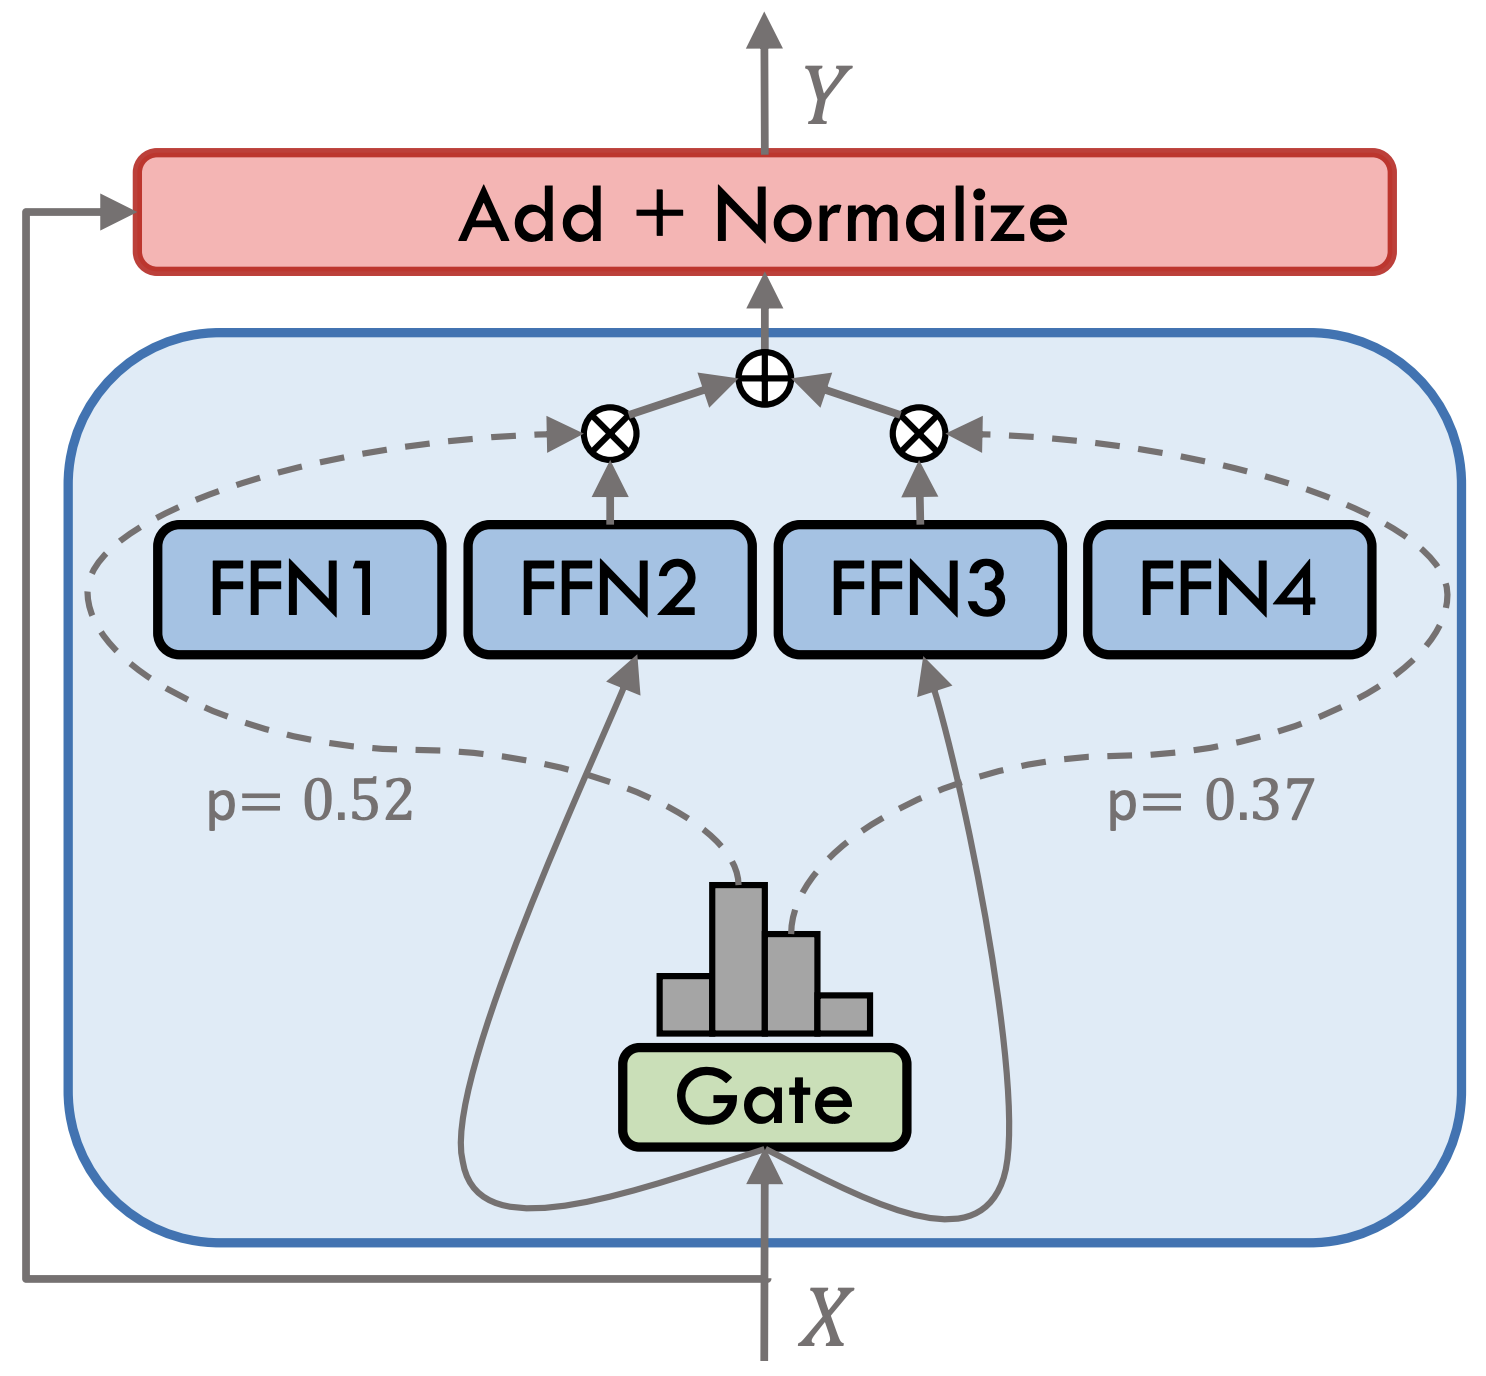
\includegraphics[width=0.6\linewidth]{figures/moe_module.jpg}
    \caption{混合专家模型层}
    \label{fig:moe_module}
\end{figure}

\section{经典Top-k路由算法}
\label{sec:classic_top-k}
路由算法是混合专家模型的心脏，其设计直接决定了模型的性能、训练稳定性以及计算效率。理想的路由算法应具备内容感知、负载均衡和计算高效等特性。目前最主流且被广泛应用的路由算法是由 Shazeer 等人\cite{Shazeer2017OutrageouslyLN}提出的基于\textbf{Top-k门控}的稀疏门控机制。对于输入词元 $\mathbf{x}$，路由器的计算过程如下：
\begin{enumerate}
    \item \textbf{（前向）计算路由Logits}: 路由器（一个线性层 $\mathbf{W}_g$）将词元 $\mathbf{x}$ 映射到维度等于专家数量 $N$ 的向量，得到路由Logits：$h(\mathbf{x}) = \mathbf{W}_g \mathbf{x}$。
    % \item \textbf{添加噪声 (可选)}: 为了在训练中促进路由决策的探索性并改善负载均衡，通常会向Logits中添加标准高斯噪声：$h(\mathbf{x})_{\text{noisy}} = h(\mathbf{x}) + \mathcal{N}(0, 1/N^2)$。
    \item \textbf{（前向）选择Top-k专家}: 从 $h(\mathbf{x})_{\text{noisy}}$ 中选取值最大的 $k$ 个维度，其对应的索引即为被选中的 $k$ 个专家的索引。具体地，在 Switch Transformer\cite{Fedus2021SwitchTS}中，$k$设置为了1，实现了极高的稀疏度（$N$最大为2048）；gpt-oss\cite{openai2025gptoss}选择了$k = 4$以及$N = 32$（20B模型）或$128$（120B模型），通过一个适中的稀疏度和较粗粒度的专家来平衡模型表现与推理效率；国内近期的大模型DeepSeek-V3\cite{DeepSeekAI2024DeepSeekV3TR}、Kimi K2\cite{Bai2025KimiKO}则分别选择了$k = 8,\ N = 256$与$k=8, N=384$，用类似gpt-oss的稀疏度但是更细粒度的专家（同等$k/N$下更大的$k$）来换取性能提升。
    \item \textbf{（前向）计算门控权重}: 对选出的 $k$ 个Logits应用Softmax函数或Sigmoid函数，生成归一化的门控权重（Gating Weights）$G(\mathbf{x})$。最初的混合专家模型以Softmax函数为主流\cite{Shazeer2017OutrageouslyLN,Lepikhin2020GShardSG,Fedus2021SwitchTS}，Sigmoid函数虽有尝试\cite{Lewis2021BASELS,Dai2022StableMoESR}，但未被广泛采用。不过，值得一提的事，近来国内开源的大模型有若干采用了Sigmoid函数作为路由器的激活函数\cite{DeepSeekAI2024DeepSeekV3TR,Bai2025KimiKO,Zeng2025GLM45AR}。
    \item \textbf{（反向）梯度直通估计 (Straight-Through Estimator)}：
    由于 \text{Top-k} 选择操作是离散且不可导的，标准的反向传播会在此处中断。为了训练路由器，模型采用了梯度直通估计（STE）\cite{Rosenblatt1958ThePA,Bengio2013EstimatingOP,Jang2016CategoricalRW,Liu2023BridgingDA}的技巧。其核心思想是，在反向传播时，我们为这个离散步骤手动定义一个“伪梯度”。我们首先考虑最终输出 $y = \sum_{i \in I} G_i(x) \cdot E_i(x)$，其中 $I$ 是被选中的 \text{Top-k} 专家索引集。梯度直通估计认为，损失 $L$ 对门控权重 $G_i$ 的梯度，只对那些被选中的专家（$i \in I$）有意义，其值与对应专家的输出 $E_i(x)$ 与输出的梯度$\frac{\partial L}{\partial y}$有关。利用多元链式法则，损失 $L$ 对标量门控权重 $G_i$ 的梯度（一个标量） ，是损失对输出向量 $y$ 的梯度（向量）与该专家输出 $E_i(x)$ （向量）的内积，亦即：
    \begin{equation}
        \frac{\partial L}{\partial G_i} = 
    \begin{cases}
        \nabla_y L \cdot E_i(x) & \quad \text{if } i \in I \\
        0 & \quad \text{if } i \notin I
    \end{cases}
    \end{equation}
    
    梯度直通估计的作用就是将这个计算出的梯度 $\frac{\partial L}{\partial G_i}$ 作为有效梯度，继续通过 Softmax 函数回传到路由器对应的 logit $h_i(x)$ 上。这样，尽管 \text{Top-k} 选择本身不可导，但路由器的参数 $W_g$ 依然能够接收到有效的学习信号并进行更新。
    
\end{enumerate}


% unfinished
\section{Top-k 路由的变体与优化}
尽管标准Top-k机制非常成功，但其局部贪心的性质可能导致次优的全局分配和负载不均衡。因此，工业界与学术界探索了多种变体以求改进。

\subsection{带随机性的Top-k路由} 
\paragraph{随机丢弃的Top-2路由} GShard\cite{Lepikhin2020GShardSG}出于负载均衡和训练推理效率的考虑，在\text{Top-2}路由中引入了依照第二个专家的概率分数（亦即对输出的权重）随机丢弃该专家的策略，丢弃的概率即$1 - G_i$。

\paragraph{带噪声的Top-k路由} 
Shazeer等人在其2017年提出的开创性工作\cite{Shazeer2017OutrageouslyLN}中引入了噪声机制，通过增加路由过程的随机性来促进负载均衡。其核心思想是在计算出的路由Logits送入Top-k选择逻辑之前，为其添加一个可学习的、与输入相关的噪声： 
\begin{equation}
h_{\text{noisy}}(x)_i = (x W_g)_i + \text{StandardNormal}() \cdot \text{Softplus}((x W{\text{noise}})_i)
\end{equation}
其中，$W_{\text{noise}}$ 是一个与路由权重矩阵 $W_g$ 相互独立的、可训练的权重矩阵，用于生成噪声的缩放因子。$\text{Softplus}$ 函数确保该因子始终为正。

值得注意的是，在如今的大语言模型中，这种随机噪声路由已经很少被采用。一方面，随机路由可能带来训练的不稳定性，增加训练噪声，降低训练效率，另一方面，随机路由也给推理部署时的表现带来了不确定性。

\subsection{全局优化的路由}
尽管经典的 \text{Top-k} 路由机制通过引入辅助损失函数能在一定程度上缓解负载不均衡问题，但这种基于启发式规则的局部优化方法仍然是影响混合专家模型性能与训练稳定性的普遍挑战。为了从根本上解决这一问题，研究者们提出了一系列全局优化的路由策略，旨在将路由过程从对单个词元的贪心决策，转变为对整个批次（batch）的整体最优分配。

\paragraph{BASE 路由}
为了实现专家间的完美负载均衡，Lewis 等人\cite{Lewis2021BASELS}提出了“稀疏专家均衡分配层”（Balanced Assignment of Sparse Experts, BASE layer）。该方法将词元到专家的分配过程重新定义为一个经典的\textbf{线性分配问题}（Linear Assignment Problem）。其核心思想是，对于一个包含 $T$ 个词元 $\{x_1, \dots, x_T\}$ 和 $N$ 个专家的批次，寻找一个分配矩阵 $\mathbf{A} \in \{0, 1\}^{T \times N}$，最大化所有词元与其被分配到的专家之间的总亲和度。目标函数可以表示为：
\begin{equation}
\max_{\mathbf{A}} \sum_{t=1}^{T} \sum_{i=1}^{N} A_{ti} \cdot h_i(x_t)
\end{equation}
其中 $h_i(x_t)$ 是路由器为词元 $x_t$ 计算的关于专家 $i$ 的亲和度得分（logit），$A_{ti}=1$ 表示将词元 $t$ 分配给专家 $i$。该优化过程受到两个硬性约束：
\begin{enumerate}
    \item $\sum_{i=1}^{N} A_{ti} = 1, \quad \forall t \in \{1, \dots, T\}$ （每个词元必须且只能被分配给\textbf{一个}专家）。
    \item $\sum_{t=1}^{T} A_{ti} = T/N, \quad \forall i \in \{1, \dots, N\}$ （每个专家必须被分配完全相同数量的词元）。
\end{enumerate}
这种方法将路由决策转化为一个全局联合优化问题，通过匈牙利算法或类似的优化求解器可以得到最优解，从而在理论上完全消除了负载不均衡以及对辅助损失函数的依赖。

\paragraph{S-BASE 路由}
Clark 等人\cite{Clark2022UnifiedSL}在 BASE 路由的基础上，引入了\textbf{最优传输}（Optimal Transport）理论，提出了 S-BASE 层。该方法将路由问题建模为寻找一个最优的“传输方案” $\mathbf{P} \in \mathbb{R}_{+}^{T \times N}$，将词元的分布（视为源）映射到专家的处理容量分布（视为目标）上。其目标是最大化总体的路由亲和度，数学上等价于最小化传输“成本”，其中成本矩阵 $\mathbf{C}$ 定义为亲和度的负值，即 $C_{ti} = -h_i(x_t)$。目标函数为：
\begin{equation}
\min_{\mathbf{P}} \sum_{t=1}^{T} \sum_{i=1}^{N} P_{ti} \cdot C_{ti} \equiv \max_{\mathbf{P}} \sum_{t=1}^{T} \sum_{i=1}^{N} P_{ti} \cdot h_i(x_t)
\end{equation}
约束条件变为概率分布上的匹配：每个词元被视为一个质量为 $1/T$ 的粒子，每个专家拥有 $1/N$ 的容量。在求解出$\mathbf{P} \in \mathbb{R}_{+}^{T \times N}$后，每个词元将被路由到对自己而言概率最高的专家。这种基于最优传输的公式概念优雅，且能够利用高效的熵正则化算法（如 Sinkhorn 算法）进行快速近似求解，从而在保持近乎完美的负载均衡的同时，提升了计算效率。

值得指出的是，这一类方法利用了全局信息进行建模，也就是需要在获取整句句子的信息的情况下进行路由，这导致这类方法更适合BERT类的编码器模型而非GPT类的解码器模型，因为后者有因果掩码（Casual Mask），句子前半部分的路由决策不能利用整句句子的全局信息。强制在GPT上使用此类方法有信息泄露的风险\cite{Clark2022UnifiedSL}，这一点和后文将要提到的，我们自己的工作\cite{Wang2024AuxiliaryLossFreeLB}中提到的Expert Choice类型的混合专家模型\cite{Zhou2022MixtureofExpertsWE}的信息泄露类似。


\subsection{基于规则的路由 (Rule-based Routing)}
与依赖于可学习参数的动态路由机制相对，另一大类路由方法采用固定的、非学习的规则来进行专家选择。这类方法的核心优势在于完全消除了路由器的训练过程，从而避免了相关的训练不稳定性和额外的参数开销，并且通常能够通过设计实现完美的负载均衡。

\paragraph{哈希路由 (Hash Routing)}
最直接的规则化路由方法是基于哈希函数，如 Hash Layers\cite{Roller2021HashLF}所提出的那样。其机制非常简单：将一个预先选定的、具有良好分布特性的哈希函数应用于每个输入词元 $x_t$（或其某种表征），然后将得到的哈希值对专家总数 $N$ 取模，从而确定该词元被分配到的专家索引：
\begin{equation}
\text{index}(x_t) = \text{hash}(x_t) \pmod N
\end{equation}
这种方法的计算开销极低，在推理时速度极快。通过选择合适的哈希函数，可以在期望上实现词元在所有专家间的均匀分布，从而达到天然的负载均衡。然而，其最主要的缺点是\textbf{语义盲目性}：路由决策完全独立于词元的语义内容，这从根本上阻止了模型根据数据模式学习出有意义的专家专业化分工。

\paragraph{带一致性约束（Consistency Regularized Loss）的随机路由}
THOR\cite{Zuo2021TamingSA}算法在训练和推理过程中，为每个输入词元随机分配两个专家。为了在这种随机性下保证模型训练的有效性，THOR 引入了一种\textbf{一致性正则化损失}（Consistency Regularized Loss）。该损失函数旨在促使被随机选中的两个专家对同一个输入的预测尽可能保持一致，从而鼓励所有专家学习到具有一定共性的、鲁棒的知识。这种方法在保证负载均衡的同时，通过引入正则化来间接引导专家的学习过程。不过，这一方法某种意义上和混合专家模型期望的专家分工相悖。

\paragraph{基于元数据的路由（Metadata-based Routing）}
这类方法利用输入数据本身附带的元信息（Metadata）作为路由的依据，实现了更具逻辑性的专家分配。
\begin{itemize}
    \item \textbf{按领域路由（Domain-based Routing）}：如图\ref{fig:DEMIX}所示，DEMix 模型\cite{Gururangan2021DEMixLD}为不同的预训练数据领域（如新闻、维基百科、代码等）显式地分配了不同的专家。在处理来自已知领域的词元时，模型会确定性地将其路由到对应的“领域专家”处。这种方式创建了清晰且可解释的专家分工。其局限性在于，当面对来自未见领域或混合领域的数据时，模型的泛化能力可能会受到影响。同时，如果在推理时无法直接获取到领域标签，那估计模型标签的步骤又会引入新的复杂度。
    \item \textbf{按语言路由（Language-based Routing）}：在多语言翻译模型中，如 M2M-100\cite{Fan2020BeyondEM}所采用的策略，路由规则可以简单地基于输入词元的语言类型。所有西班牙语的词元被送往“西班牙语专家”，所有法语词元则送往“法语专家”。特别地，一些训练数据较少的语言被按照相似度分组聚合成若干的专家。特别地，为了让不同专家能够学习到不同语言中共通的部分，作者也引入了随机性路由，使得一种专家有希望见到别的语言的数据。
\end{itemize}
基于元数据的路由虽然能够实现有意义的专家分工，但其灵活性较差，且专家的划分粒度完全依赖于预先定义的元数据类别。

\begin{figure}[h]
    \centering
    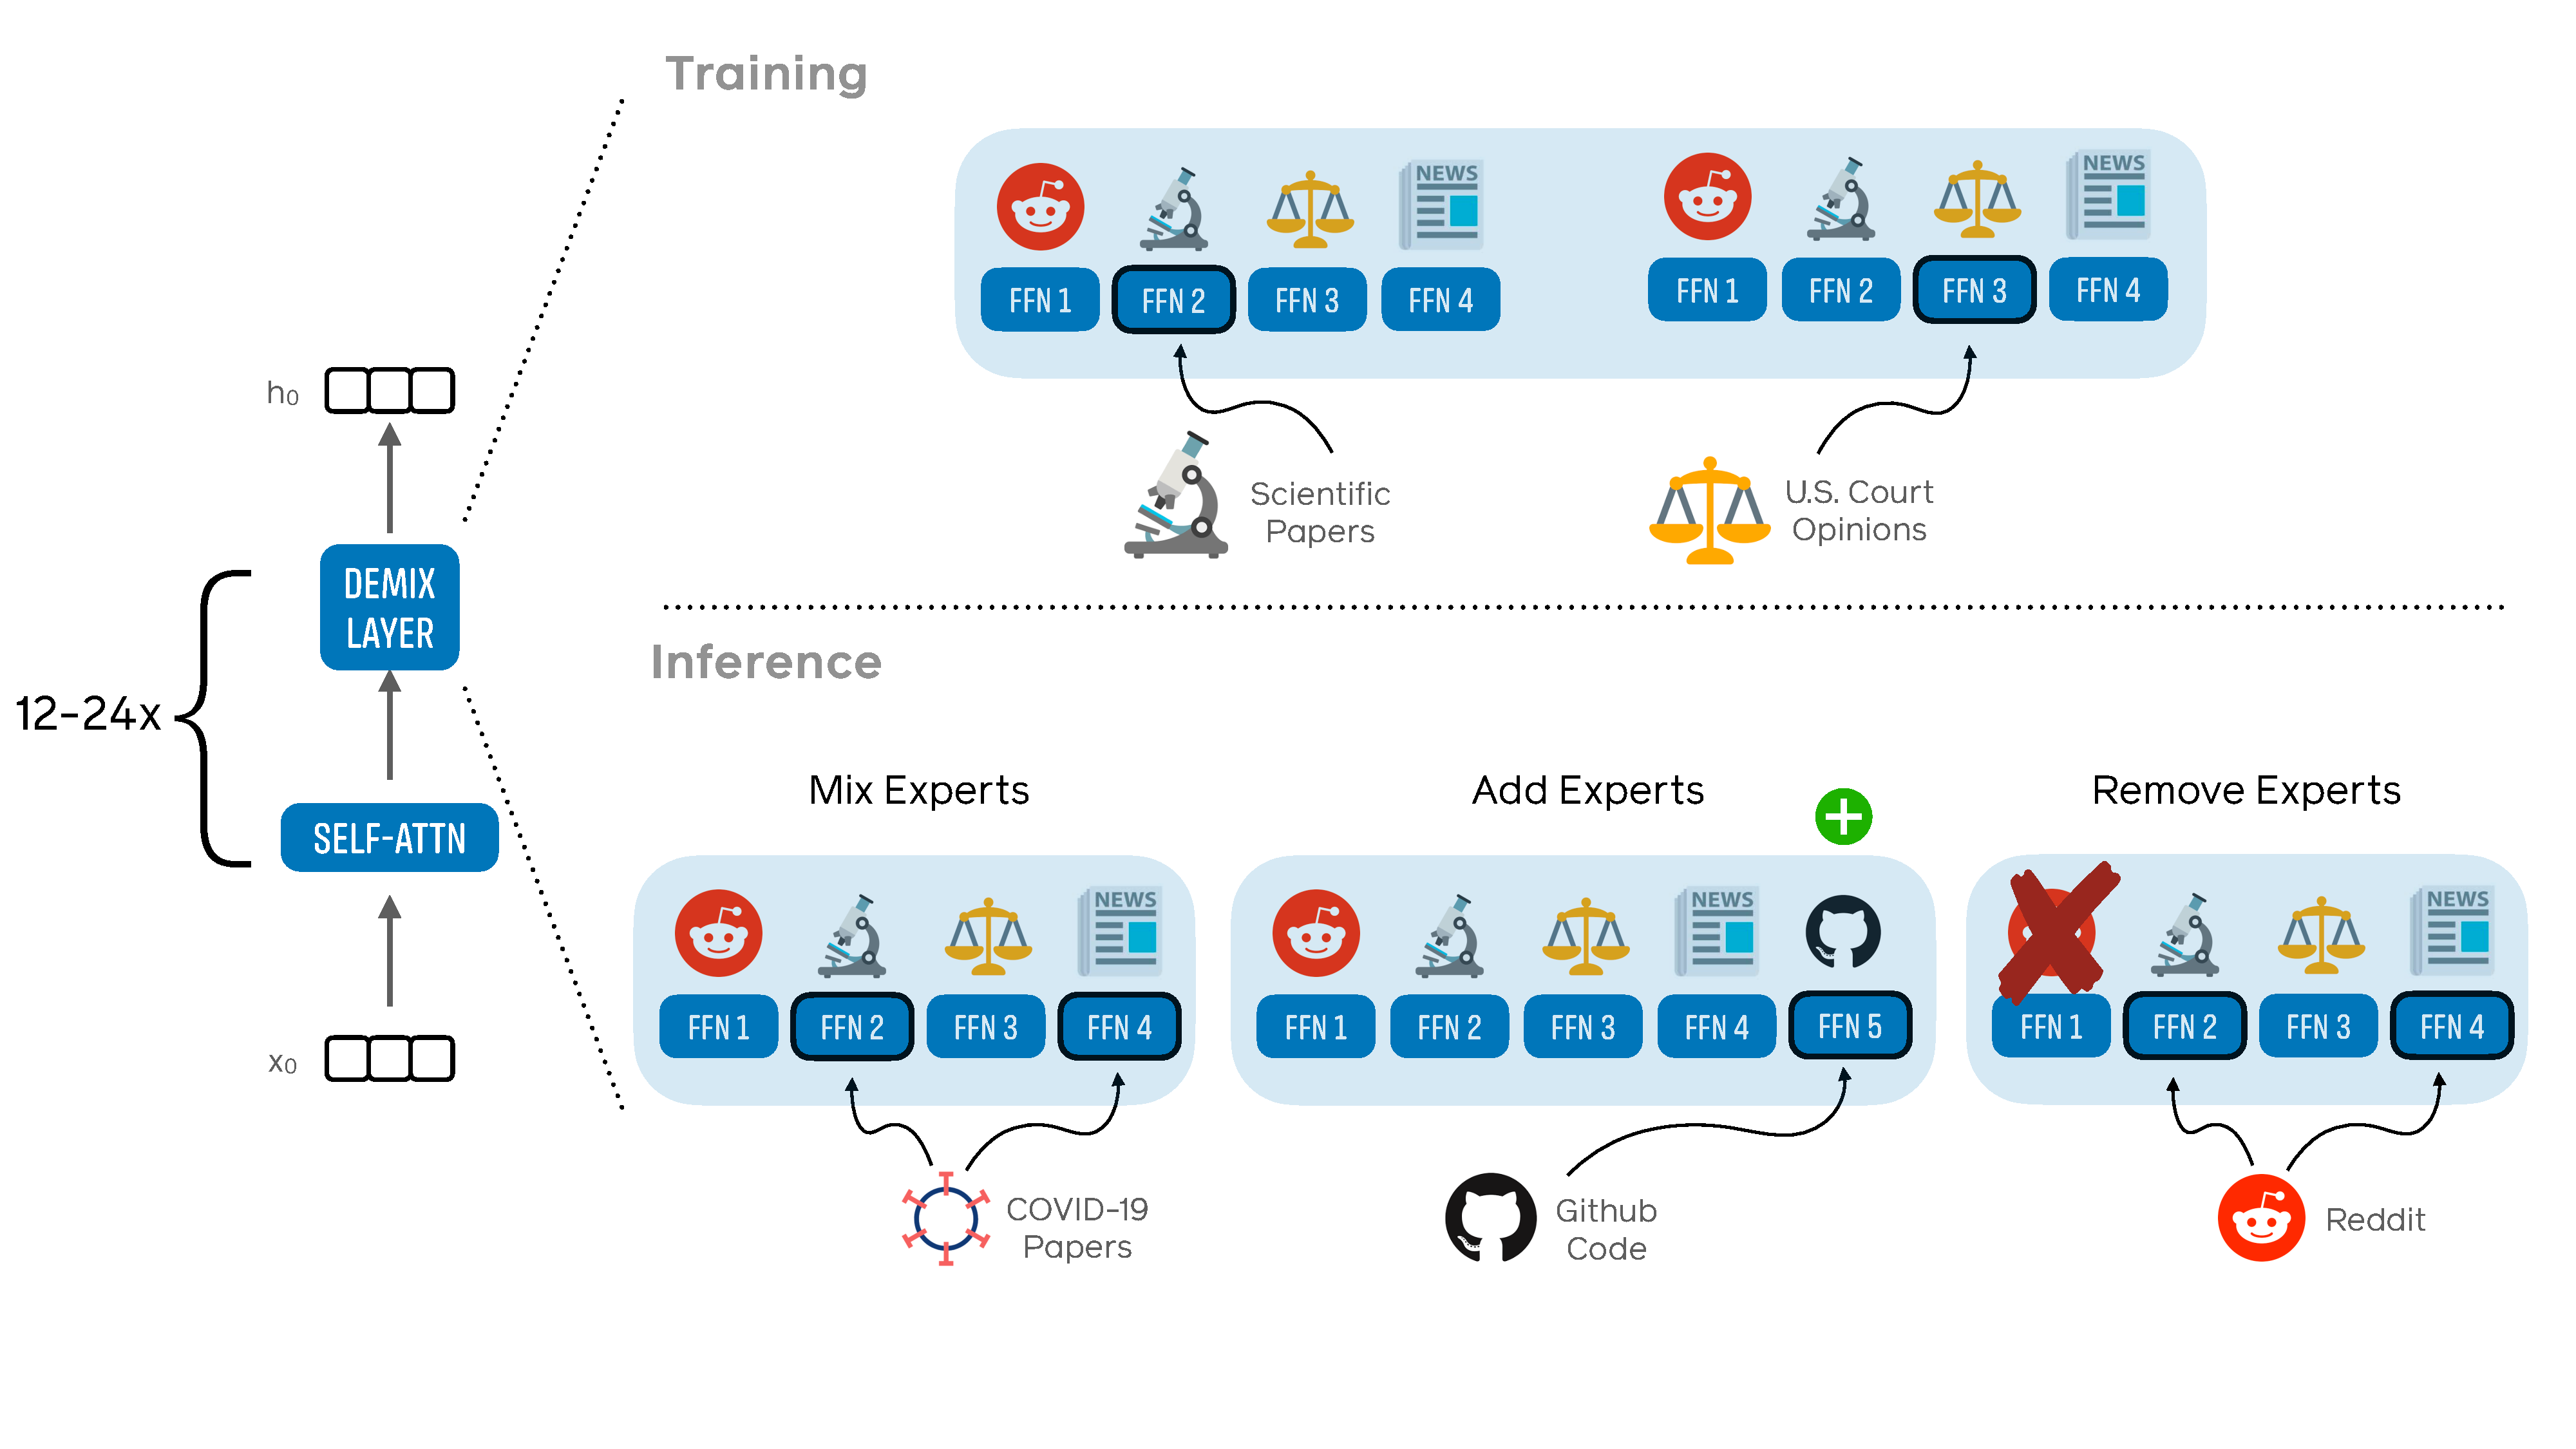
\includegraphics[width=1.0\linewidth]{figures/DEMIX.pdf}
    \caption{DEMix 模型\cite{Gururangan2021DEMixLD}为不同的预训练数据领域显式地分配了不同的专家。}
    \label{fig:DEMIX}
\end{figure}


\paragraph{混合路由策略（Hybrid Routing Strategies）}
为了结合不同规则化路由的优点，研究者们还提出了混合策略。例如，PanGu-$\Sigma$\cite{Ren2023PanGuTT}模型采用了一种两阶段的路由机制（图\ref{fig:hybrid_domain_hash}）：首先，根据词元所属的领域，将其确定性地路由到一个特定的\textbf{专家组}；然后，在该专家组内部，再通过随机选择的方式确定最终处理该词元的单一专家。这种“先按领域分组，再组内随机”的混合策略，既利用了元数据带来的语义引导，又保留了随机路由的简洁性和负载均衡特性。

\begin{figure}[h]
    \centering
    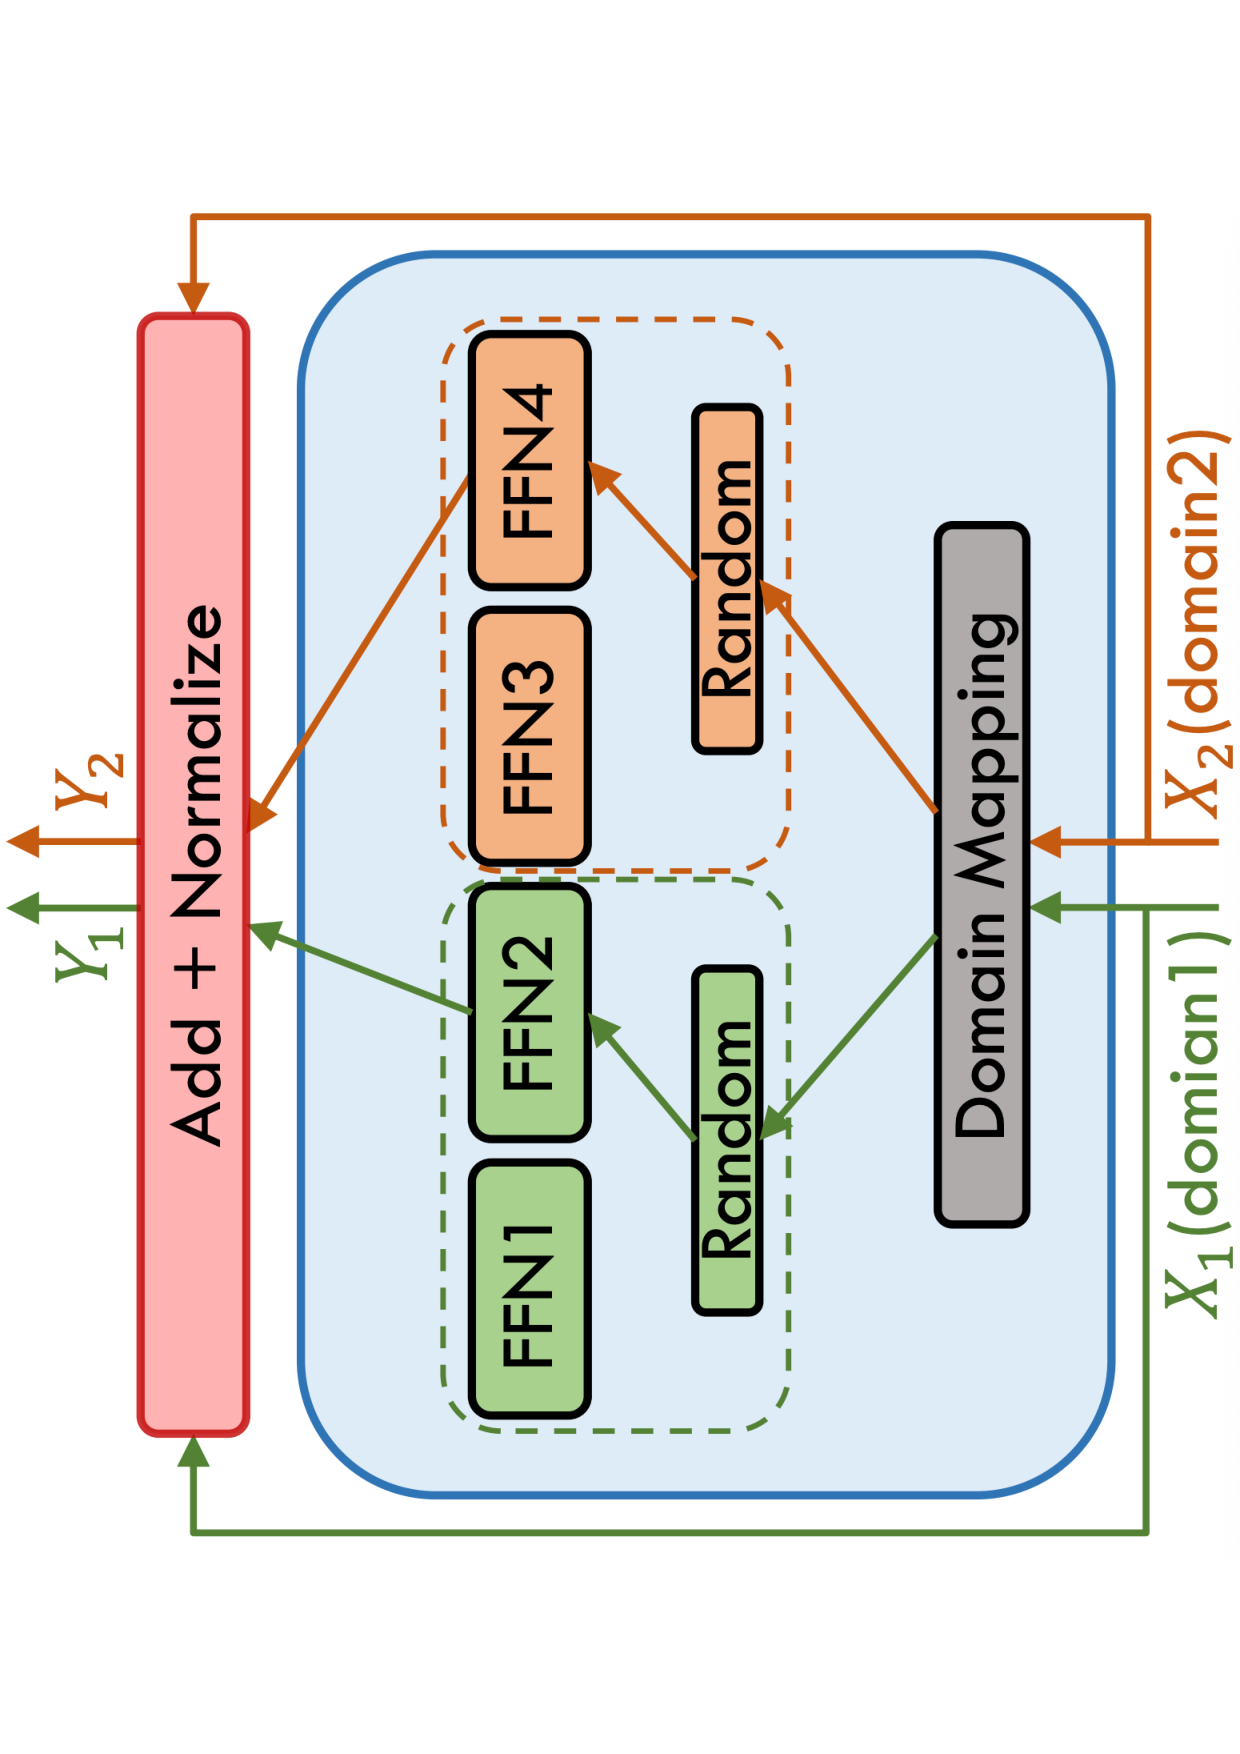
\includegraphics[angle=-90,width=0.8\linewidth]{figures/hybrid_domain_hash.pdf}
    \caption{PanGu-$\Sigma$\cite{Ren2023PanGuTT}模型的两阶段路由机制}
    \label{fig:hybrid_domain_hash}
\end{figure}


从某种意义上说，基于规则的路由相当于使用基于人类先验的路由策略替代了基于数据驱动学习的路由策略。它在特定场景下能够发挥一定的作用，也有着实现简单、负载均衡好的优点。然而，对于当前面临复杂多变应用场景的大语言模型而言，仅依赖此种单一策略恐显不足。

\subsection{路由器的变种}
经典的路由器采用一个简单的线性变换层后接 \text{Softmax}（或Sigmoid） 和 \text{Top-K} 算子来计算门控权重。为了进一步捕捉输入词元与专家功能之间的复杂关系，提升路由决策的质量和模型的整体性能，研究者们探索了多种相对更复杂的路由器的变种。

\paragraph{余弦路由器（Cosine Router）}
研究发现，经典的线性路由器存在一个潜在的严重问题，即\textbf{表示坍缩}（Representation Collapse）\cite{Chi2022OnTR}。具体而言，在线性路由机制下，为了获得较高的路由得分（logits），模型倾向于将输入词元的隐藏表示（hidden representations）推向与路由器权重向量（可视为专家质心）在空间中极为接近的位置。这种优化压力导致所有词元的表示都向少数几个专家质心聚集，失去了多样性和表达能力，从而损害了模型的整体性能。
为了缓解这一问题，Chi 等人提出采用\textbf{余弦路由器}。其核心思想是将路由决策从基于向量点积的亲和度，转变为基于向量方向的余弦相似度。这通过将词元表示和专家嵌入都投影到一个单位超球面上来实现，从而解耦了向量的\textbf{幅值}（magnitude）与路由得分的关系。路由决策仅依赖于两者之间的夹角，而向量的幅值则可以被模型用于编码其他维度的信息，从而保留了表示的多样性。其门控函数 $G(\mathbf{x})$ 的计算过程如下：
\begin{equation}
G(\mathbf{x}) = \text{TopK} \left( \text{softmax} \left( \tau \cdot \frac{(\mathbf{W}_{\text{linear}}\mathbf{x})^T \mathbf{C}}{\|\mathbf{W}_{\text{linear}}\mathbf{x}\| \|\mathbf{C}\|} \right) \right)
\end{equation}
其中，$\mathbf{x}$ 是输入词元的表示，$\mathbf{W}_{\text{linear}}$ 是一个可学习的线性投影矩阵。$\mathbf{C} \in \mathbb{R}^{d_{model} \times N}$ 代表了 $N$ 个专家的可学习嵌入向量。核心计算部分即为投影后的词元表示与各个专家嵌入之间的余弦相似度。$\tau$ 是控制分布锐利度的温度参数。通过这种方式，余弦路由器有效防止了表示坍缩，鼓励模型学习到更具信息量的特征表示，并在领域泛化等任务上展现出一定的优势。

\paragraph{注意力路由器 (Attention Router)}
为了设计一个能够更有效捕捉词元与专家之间亲和度的路由机制，Yuan 2.0-M32 模型\cite{Wu2024Yuan2M}引入了\textbf{注意力路由器}（Attention Router）。如图\ref{fig:attention_router}所示，该设计将标准注意力机制的思想应用于路由过程，取代了简单的线性层，从而实现了更具动态性和语义感知能力的专家选择。其详细工作流程如下：
\begin{enumerate}
    \item \textbf{输入投影}：与标准自注意力模块类似，输入的单个词元表征 $\mathbf{x}$ 首先被线性投影，生成三组d维向量，每组N（专家数目）个，对应于查询（Query）、键（Key）和值（Value）向量：
    \begin{equation}
    \mathbf{Q} = \mathbf{W}_Q \mathbf{x}, \quad \mathbf{K} = \mathbf{W}_K \mathbf{x}, \quad \mathbf{V} = \mathbf{W}_V \mathbf{x}
    \end{equation}
    \item \textbf{注意力计算}：查询（Query）、键（Key）和值（Value）三组向量按照注意力机制计算出一个N维输出向量$\mathbf{P}$，表示该词元与每个专家的相关性：
    \begin{equation}
    \mathbf{P} = \text{softmax}\left(\mathbf{Q} \mathbf{K}^T\right)\mathbf{V}
    \end{equation}
    \item \textbf{专家选择}：选取N维输出向量$\mathbf{P}$中前$K$大的分数对应的专家。
\end{enumerate}
这种设计允许路由器在做出最终路由决策前，进行一次丰富的特征交互。它不仅考虑了词元自身的属性，还动态地融入了该词元与整个专家池的关联信息，从而实现了比简单线性映射更复杂的专家选择。在Yuan 2.0-M32中，$K=2, N=32, d=2048$。

\paragraph{平均键路由器 (Avg-K Router)}
Liu 等人提出\cite{Liu2023TowardsAU}，可以将混合专家模型（MoE）的 Transformer 层看作一个拥有巨大尺寸的、被分块的键值对记忆网络（Key-Value Memory Network）。在这个视角下，每个专家（Expert）本质上是一个独立的记忆块（Memory Block），包含了若干键（Key）和值（Value）向量对，而前馈网络（FFN）的计算过程可以被视为一种记忆检索和整合的过程。一个标准的前馈网络计算可以表示为：
\begin{equation}
    y = \text{FFN}(x) = f(x \cdot K^T) \cdot V
\end{equation}
其中 \(x\) 是输入，\(K\) 和 \(V\) 分别是前馈网络的两个线性层的权重，可以被看作是记忆的键表和值表。
从这个角度出发，经典的混合专家模型路由器在选择专家时，使用的是一个独立于专家内部参数（即键 \(K\)）的门控网络。这种分离可能导致路由决策与专家的实际功能存在偏差。
为了将路由决策与专家的内在功能更紧密地联系起来，Liu 等人提出了 \textbf{Avg-K} 路由方法。该方法直接利用每个专家（记忆块）自身的键向量来决定路由。其核心思想是，用每个记忆块中所有键向量的平均值来代表这个记忆块。具体算法如下：
\begin{enumerate}
    \item \textbf{计算专家代表向量}：对于第 \(i\) 个专家，其代表向量 \(e_i\) 由该专家内部的所有键向量 \(k_j^{(i)}\) 的平均值计算得出。假设每个专家（记忆块）的大小为 \(g\)，则：
    \begin{equation}
        e_i = \text{Avg}(\mathbf{K}^{(i)}, \text{dim=0}) = \frac{1}{g} \sum_{j=0}^{g-1} k_j^{(i)}
    \end{equation}
    其中 \(\mathbf{K}^{(i)}\) 是第 \(i\) 个专家的键矩阵。
    \item \textbf{计算路由得分}：输入词元 \(x\) 与每个专家的代表向量 \(e_i\) 计算点积，得到路由得分。
    \begin{equation}
        \text{score}_i = x \cdot e_i
    \end{equation}
    \item \textbf{专家选择}：根据计算出的得分，选择得分最高的 \(b\) 个专家进行激活。
\end{enumerate}
由于平均操作的线性特性，计算输入 \(x\) 与平均键向量的点积，等价于计算 \(x\) 与该专家内所有键向量的点积然后取平均值。这种设计直接利用了专家的键信息，增强了路由决策的依赖性，从而获得了较好的性能。

\begin{figure}[h]
    \centering
    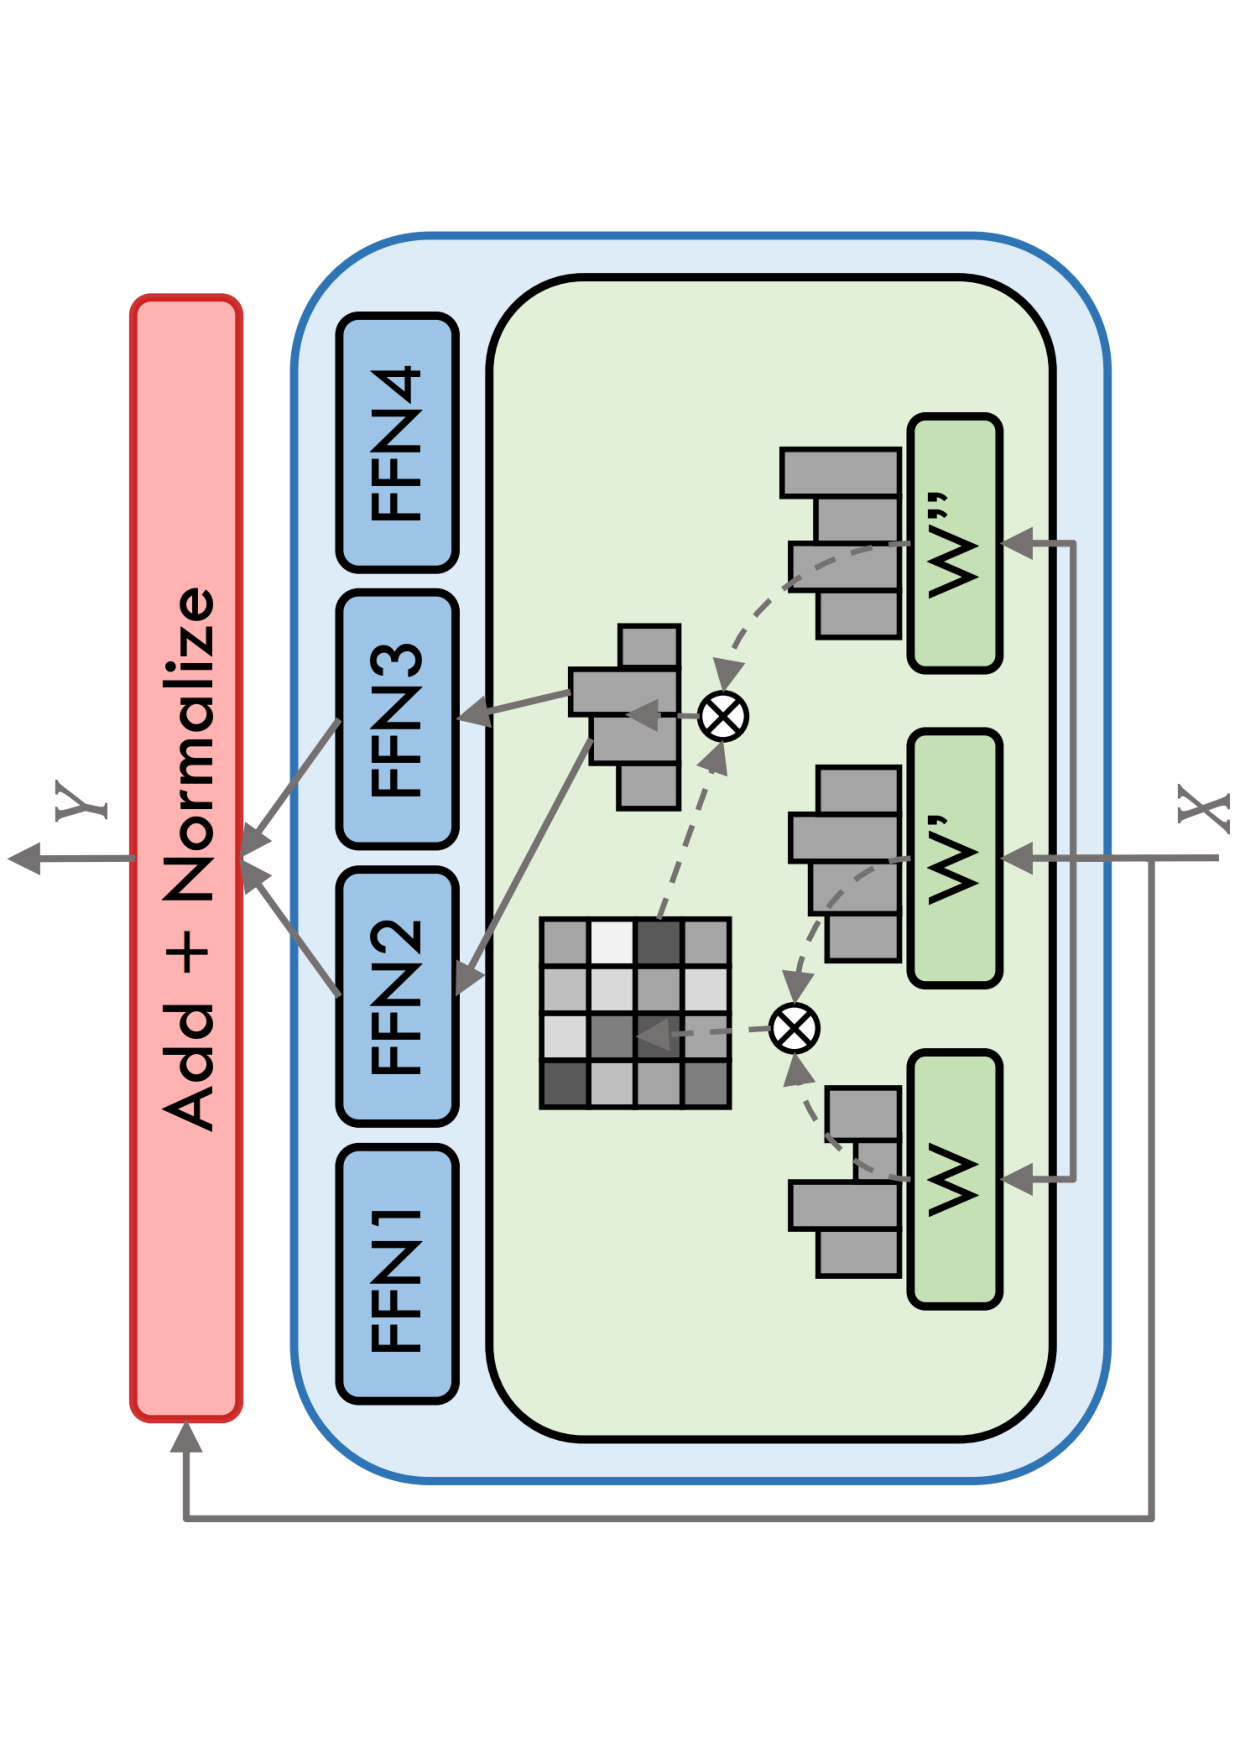
\includegraphics[angle=-90,width=0.8\linewidth]{figures/attention_router.pdf}
    \caption{注意力路由器}
    \label{fig:attention_router}
\end{figure}

\subsection{路由器的学习算法}
\label{sec:router_learning}
路由器的参数 $W_g$ 对于混合专家模型的性能至关重要，因为它直接决定了每个输入词元应该由哪些专家进行处理。然而，如 \ref{sec:classic_top-k} 所述，Top-k 选择操作本身是离散的、不可导的，这为通过标准的反向传播算法来训练路由器带来了挑战。为了解决这个问题，研究者们借鉴了强化学习和数值方法等领域的思想，提出了一系列新颖的学习算法。

\paragraph{REINFORCE 算法及其变种}
REINFORCE\cite{Williams2004SimpleSG}是一种经典的策略梯度方法，常用于优化随机策略网络。在混合专家模型的上下文中，可以将路由器的决策过程视为一个策略：对于给定的输入词元 $x$，路由器选择一个或多个专家的动作\cite{Clark2022UnifiedSL}。REINFORCE 算法的核心思想是通过最大化期望奖励来更新策略参数。
具体来说，REINFORCE 梯度估计器在理论上是无偏的，并且只要求离散变量的分布是可导的，而不需要通过模型的其余部分 $g$ 进行反向传播。其梯度估计的形式如下：
\begin{equation}
\nabla_{\text{REINFORCE}} := g(\pi_D f_D(x)) \frac{\partial \log \pi_D}{\partial W_r}
\end{equation}
其中 $D$ 是被选择的专家，$g(\pi_D f_D(x))$ 可以被看作是选择专家 $D$ 后获得的奖励 (reward)。尽管 REINFORCE 算法在理论上是无偏的，即其梯度估计的期望等于真实的梯度，但它在实践中往往存在高方差的问题。
为了解决 REINFORCE 算法固有的高方差问题，研究者们提出了一系列基于控制变量 (control variates) 的改进方法。这些方法的核心思想是从原始的梯度估计中减去一个期望为零的随机变量，从而在不改变梯度期望（保持无偏性）的前提下，有效降低其方差。例如，MuProp\cite{Gu2015MuPropUB}使用了基于函数泰勒展开的控制变量；REBAR\cite{Tucker2017REBARLU}则巧妙地将低方差但有偏的估计器与 REINFORCE 相结合，构建出一个既无偏又低方差的梯度估计器；Grathwohl等人\cite{Grathwohl2017BackpropagationTT}更是提出通过训练一个独立的神经网络来学习最优的控制变量，以最大程度地降低方差。

\paragraph{SparseMixer 算法}
为了克服梯度直通估计 (Straight-Through Estimator, STE) 需要密集计算所有专家输出的限制，同时为被忽略的梯度项提供更可靠的估计，Liu 等人提出了 SparseMixer 算法\cite{liu2023sparsebackpropagationmoetraining}。该算法基于数值常微分方程 (ODE) 求解器的思想，旨在以一种可扩展的方式，为路由器提供更精确的梯度近似，且计算开销较小。SparseMixer 的核心思想是将路由器的梯度计算问题重新构建为一个数值积分问题。具体来说，损失函数关于路由器参数的梯度可以分为两部分 $\nabla_0$ 和 $\nabla_1$。其中 $\nabla_1$ 可以通过标准的反向传播计算，而 $\nabla_0$ 包含了与路由概率 $\pi$ 相关的项，这部分梯度的计算是难点所在。SparseMixer 提供了一种有效的方法来近似 $\nabla_0$。该算法利用了二阶 ODE 求解器，特别是中点法 (mid-point method)，来提供比传统一阶方法（如前向欧拉法，这可以看作是 STE 的一种理论解释）更精确的梯度近似。SparseMixer 的二阶版本（SparseMixer-2nd）的梯度估计形式如下：
\begin{equation}
\nabla_{\text{SparseMixer-2nd}} := 2 \cdot \frac{\partial g(\frac{\pi_D}{2} f_D(x))}{\partial W_r}
\end{equation}
其中，$D$ 是被选择的专家，$f_D(x)$ 是其输出，$g(\cdot)$ 代表模型的其余部分，$\pi_D$ 是路由到该专家的概率，$W_r$是路由器的线性变换矩阵。 这种方法在不引入 Hessian 矩阵或其他二阶导数的情况下，达到了二阶精度，并且重要的是，它只需要被激活专家的输出，从而保持了计算的稀疏性。在Liu等人的实验中，将 SparseMixer 应用于 Switch Transformer 等模型，可以显著提升性能，将训练收敛速度提升两倍。

\paragraph{Router z-loss}
在改进梯度估计算法本身以外，Zoph 等人在其 ST-MoE 的工作中提出了一种名为“Router z-loss”的辅助损失\cite{Zoph2022STMoEDS}，旨在控制路由器输出的 logits 的范围，避免logits位于浮点数精度较低的区间（也就是浮点数绝对值过大的位置）。其定义如下：
\begin{equation}
L_z = \frac{1}{T} \sum_{t=1}^{T} (\log \sum_{i=1}^{N} e^{h_i(x_t)})^2
\end{equation}
其中 $T$ 是批次中的词元总数，$N$ 是专家数量，$h_i(x_t)$ 是路由器为第 $t$ 个词元分配给第 $i$ 个专家的 logit。
这个损失函数会惩罚那些具有较大幅度的 logits，因为它会促使 $\sum e^{h_i(x_t)}$ 的值变大。在较大规模的混合专家模型上，这一辅助损失有利于促进训练稳定性。

\paragraph{两阶段稳定路由策略 (StableMoE)}
StableMoE\cite{Dai2022StableMoESR}认为，依赖学习的路由方法普遍存在\textbf{路由抖动 (routing fluctuation)} 的问题，即在训练过程中，同一个输入词元在不同阶段会被分配给不同的专家。这种不稳定性损害了样本效率，因为模型在多个专家上更新了参数，但在推理时仅使用最终确定的一个专家。为了解决此问题，StableMoE提出了一种两阶段训练策略，旨在学习一个稳定且高效的路由策略（图\ref{fig:stable_moe}）。
\begin{itemize}
    \item \textbf{第一阶段：学习与蒸馏}。在此阶段，模型采用标准的“学习路由”范式，通过优化任务损失和负载均衡损失来训练一个路由策略。与此同时，模型将这个动态学习到的、依赖于骨干网络深度表征的路由策略，通过\textbf{知识蒸馏 (knowledge distillation)} 的方式，提炼到一个与骨干网络解耦的、轻量级的\textbf{蒸馏路由器 (distilled router)}中。这个轻量级路由器通常仅使用词元的浅层表征（如词嵌入）作为输入，其学习目标是模仿主路由器的路由决策。此阶段的总损失函数为：
    $$ L_{S1} = L_{task} + L_{bal} + L_{dis} $$
    其中 $L_{task}$ 是主任务损失，$L_{bal}$ 是负载均衡损失，$L_{dis}$ 是蒸馏损失（通常为交叉熵）。
    \item \textbf{第二阶段：基于稳定路由的学习}。在第一阶段结束后，将蒸馏路由器的参数\textbf{冻结}。在整个第二阶段的训练中，所有词元的专家分配完全由这个固定的、轻量级的路由器决定。由于路由策略不再变化，路由抖动问题被彻底消除。此时，模型不再需要负载均衡和蒸馏损失，训练目标仅为主任务损失：
    $$ L_{S2} = L_{task} $$
\end{itemize}
这种两阶段方法通过先学习再固化的方式，成功地为混合专家模型提供了一个稳定、一致的路由机制，在保证路由质量的同时，提升了训练的稳定性和最终的模型性能。

\begin{figure}[h]
    \centering
    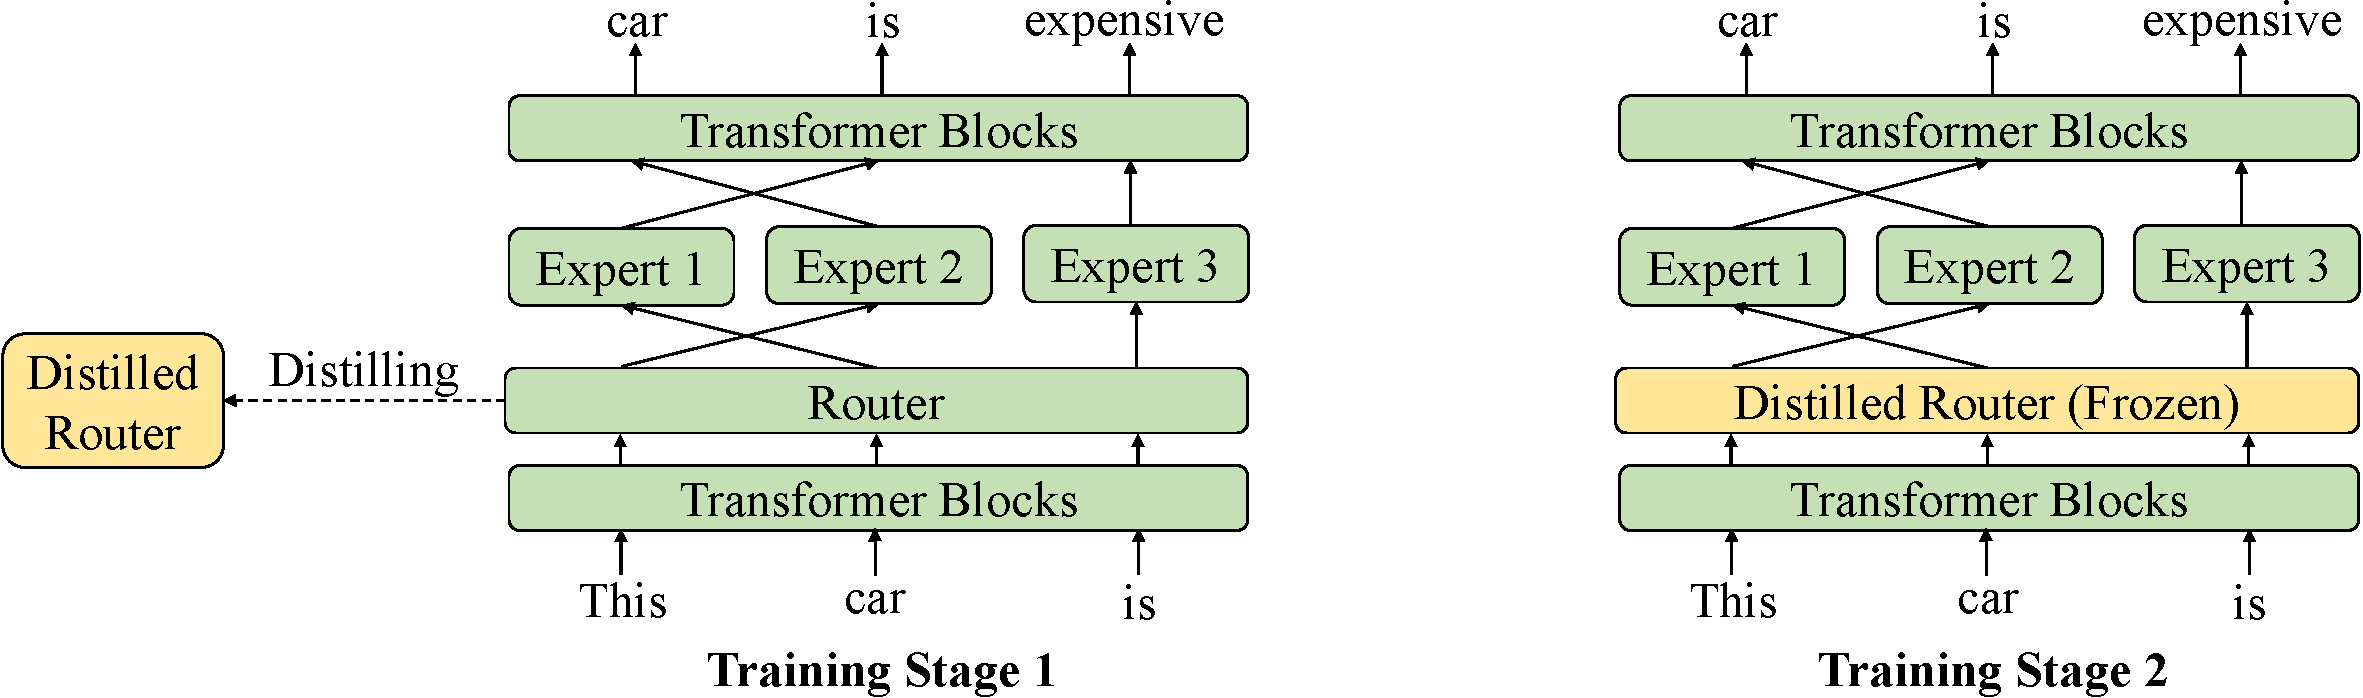
\includegraphics[width=1.0\linewidth]{figures/stable_moe.pdf}
    \caption{StableMoE的两阶段路由策略\cite{Dai2022StableMoESR}}
    \label{fig:stable_moe}
\end{figure}

\paragraph{专家自主路由 (Autonomy-of-Experts, AoE)}
经典路由机制的一个核心挑战是\textbf{决策与执行的分离}\cite{Lv2025AutonomyofExpertsM}：路由器负责预测哪个专家最适合处理输入，但它无法直接评估专家处理该输入的实际能力。这种分离可能导致次优的专家选择。
为了解决这一根本性问题，专家自主路由 (Autonomy-of-Experts, AoE)\cite{Lv2025AutonomyofExpertsM} 提出了一种全新的范式：\textbf{移除独立的路由器，让专家自主决定是否处理输入}（图\ref{fig:AOM}）。其核心思想是，一个专家对其自身处理特定词元的能力是有感知的，这种感知体现在其内部的激活向量的范数上。
具体机制如下：
\begin{enumerate}
    \item \textbf{初步计算与激活评估}。对于每个输入词元 $x$，MoE层中的\textit{所有}专家都对其执行一个低成本的初步前向计算。然后，基于该计算得到的激活的\textbf{范数}（如 L2 范数）来评估每个专家的“胜任度”。激活范数越大，代表该专家被该输入“激活”的程度越高，也就越适合处理它。

    \item \textbf{自主选择与执行}。根据所有专家的激活范数对它们进行排序，只有排名最高的$K$个专家会继续完成剩余的计算流程，而其他专家则中止计算。最终的输出由这$K$个被激活专家的结果加权组合而成。
\end{enumerate}
为了保证初步计算的效率，AoE采用了\textbf{权重矩阵的低秩分解 (low-rank factorization)}。例如，专家的第一个前馈网络权重 $W_1$ 被分解为两个低秩矩阵 $W_{down} \in \mathbb{R}^{d_{model} \times d_{low}}$ 和 $W_{up} \in \mathbb{R}^{d_{low} \times d_{ffn}}$。这样，第 $i$ 个专家的选择分数 $p_i$ 可以高效地计算：
$$ p_i = \left\| x W_{down, i} \right\|_2 $$
其中 $x W_{down, i}$ 的计算开销远小于完整的 FFN 计算。被选中的专家可以复用这个已经计算出的低维激活，继续后续的计算。
通过这种方式，AoE将路由决策权交还给专家自身，使其基于实际的内部状态进行自主选择，从而实现了更精准的专家分配和更有效的学习。


\begin{figure}[h]
    \centering
    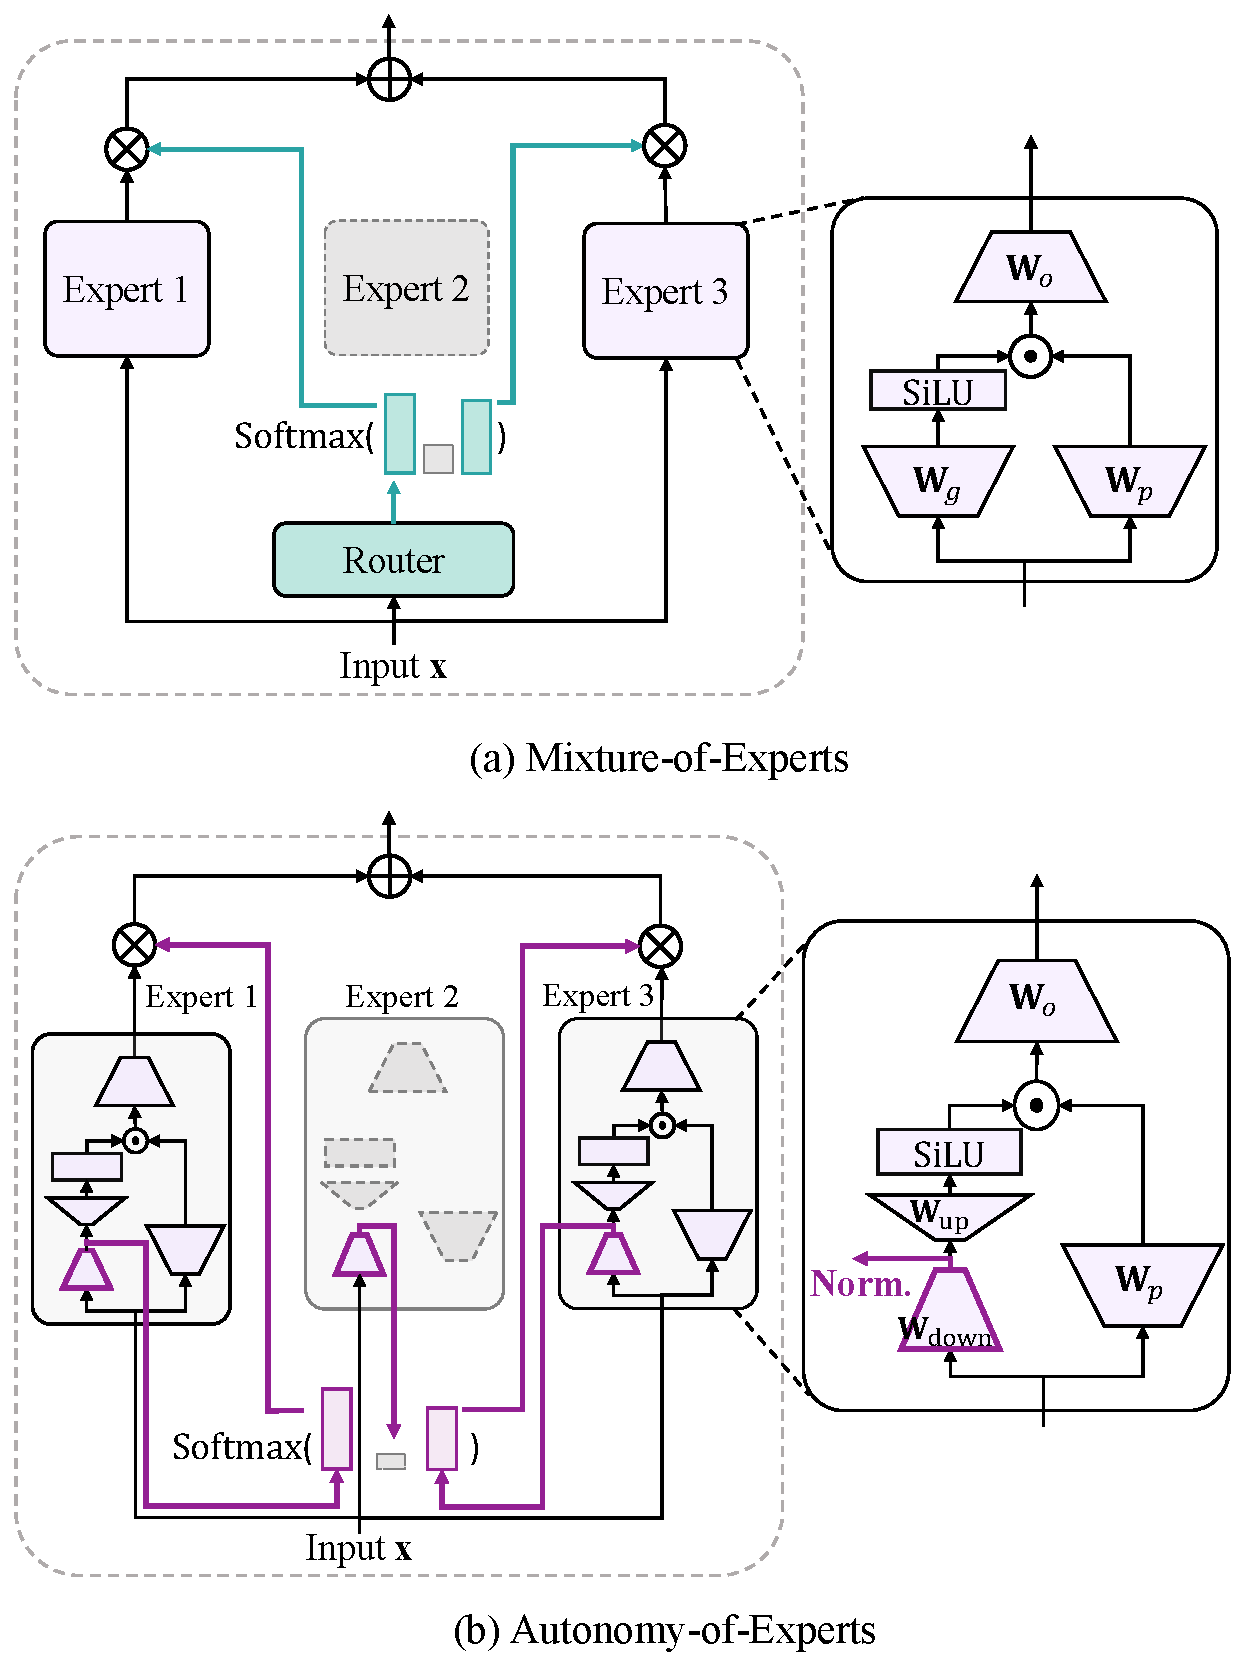
\includegraphics[width=0.7\linewidth]{figures/AOM.pdf}
    \caption{AOE与普通混合专家模型的对比\cite{Lv2025AutonomyofExpertsM}}
    \label{fig:AOM}
\end{figure}

\subsection{异构专家设计 (Heterogeneous Expert Design)}
经典的混合专家模型通常采用同质专家网络（Homogeneous Experts），即所有专家的网络结构和参数量都相同。然而，输入序列中的不同词元的计算复杂性存在差异，使用相同规模的专家处理所有词元可能导致计算资源的次优分配。为了解决这一问题，近期研究开始探索异构专家设计，通过引入不同类型或规模的专家来提升模型的效率和性能。

\paragraph{\raisebox{0.05ex}{\scalebox{0.96}{$\mathbf{\mathcal{A}}$}}\textit{da}\raisebox{0.04ex}{\textsc{\scalebox{0.85}{MoE}}}\xspace}
为了实现更灵活的路由机制，\raisebox{0.05ex}{\scalebox{0.96}{$\mathbf{\mathcal{A}}$}}\textit{da}\raisebox{0.04ex}{\textsc{\scalebox{0.85}{MoE}}}\xspace\cite{Zeng2024AdaMoETR} 提出了\textbf{空专家} (Null Experts) 的概念。其核心思想是在原有的 $n$ 个“真”专家之外，额外增加 $m$ 个空专家（图\ref{fig:adamoe}）。空专家的计算过程是一个恒等或零映射，不产生任何计算开销（FLOPs）。同时，路由器的 Top-k 选择机制中的 $k$ 值被放大到一个更大的值 $k' (k' > k)$。这样，当一个词元被路由时，其选择的 $k'$ 个专家中可能包含若干空专家。最终，该词元实际只由被选中的真专家处理，从而实现了每个词元可以自适应地激活可变数量的真专家，打破了传统混合专家模型中每个词元必须激活固定$k$个专家的限制。

\begin{figure}[h]
    \centering
    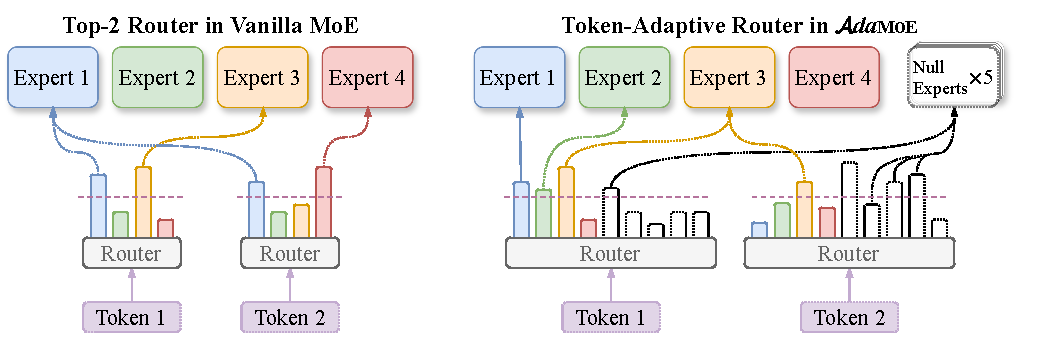
\includegraphics[width=1.0\linewidth]{figures/admoe.pdf}
    \caption{{\raisebox{0.05ex}{\scalebox{0.96}{$\mathbf{\mathcal{A}}$}}\textit{da}\raisebox{0.04ex}{\textsc{\scalebox{0.85}{MoE}}}\xspace}的示意图\cite{Zeng2024AdaMoETR}}
    \label{fig:adamoe}
\end{figure}

\paragraph{MoE++}
MoE++ \cite{Jin2024MoEAM} 框架（图\ref{fig:moe++}）引入了更丰富的\textbf{零计算专家} (Zero-Computation Experts) 来实现灵活的计算分配。具体包括三种类型：(1) \textbf{零专家 (Zero Expert)}，直接丢弃输入，输出为零向量；(2) \textbf{拷贝专家 (Copy Expert)}，直接复制输入作为输出，功能类似于残差连接；(3) \textbf{常数专家 (Constant Expert)}，用一个可训练的向量替换输入。这些设计使得简单的词元可以选择计算开销极低的路径，而将宝贵的前馈网络专家资源留给更复杂的词元。此外，MoE++还引入了\textbf{门控残差} (Gating Residuals) 机制，将上一层的路由分数作为当前层路由计算的一部分，使得路由决策能够感知词元在网络中的历史路径。

\begin{figure}[h]
    \centering
    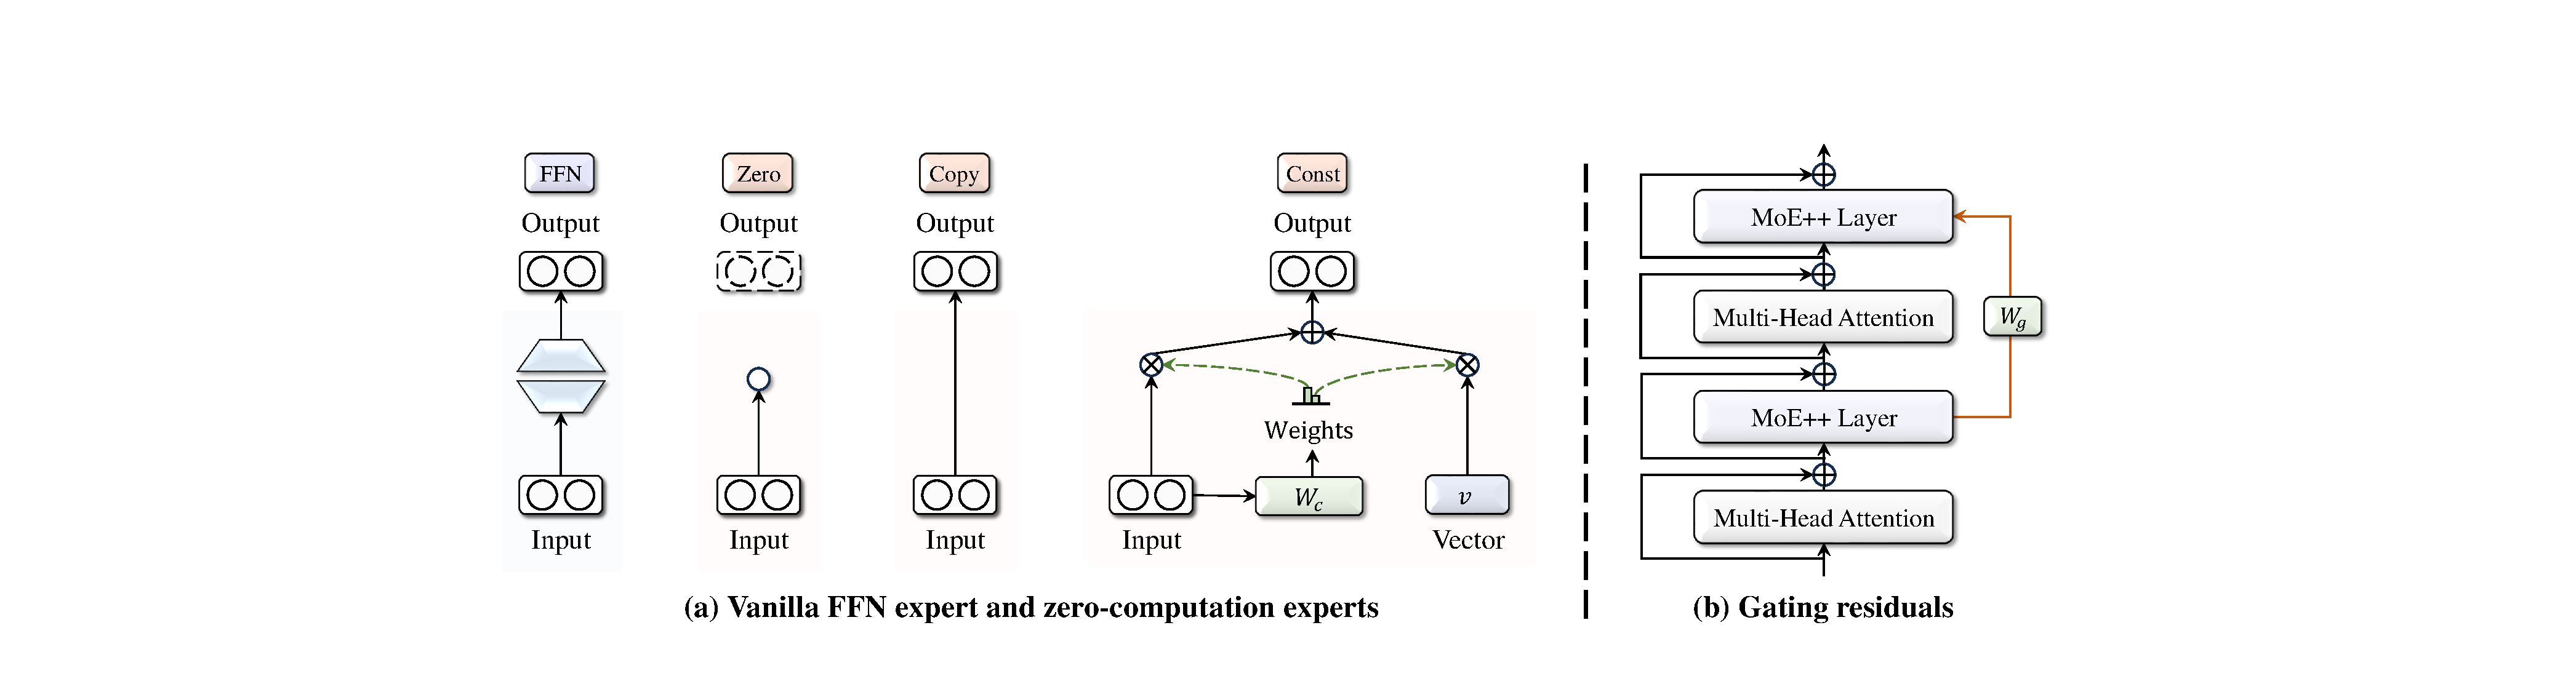
\includegraphics[width=1.0\linewidth]{figures/moe++.pdf}
    \caption{MoE++中的（a）不同类型专家和（b）门控残差机制的示意图\cite{Jin2024MoEAM}}
    \label{fig:moe++}
\end{figure}

\paragraph{HMoE}
HMoE (Heterogeneous Mixture of Experts) \cite{Wang2024HMoEHM} 模型为每个专家设置了不同的隐藏层维度，从而构建了大小各异的专家网络（图\ref{fig:hmoe}）。其核心思想是，让模型能够为复杂的词元分配计算能力更强的大专家，而为简单的词元分配计算开销较小的小专家。然而，这种设计面临一个挑战：在训练过程中，模型会倾向于频繁激活性能更优的大专家，导致小专家得不到充分训练。为解决此问题，HMoE 引入了一种新的\textbf{参数惩罚损失} (Parameter Penalty Loss)，在经典的负载均衡损失基础上，根据专家的大小对其激活进行加权惩罚。该损失函数的形式如下：
\begin{equation}
    L_{\text{P-Penalty}} = N \sum_{i=1}^{N} M_i \cdot P_i
\end{equation}
其中，$M_i$ 是专家 $i$ 在整个批次中被激活的频率乘以隐藏层维度，$P_i$ 是专家 $i$ 从路由器获得的平均门控权重。该损失函数会惩罚对大专家的过度激活，引导模型更经济地使用小专家，从而在专家之间形成更高效的功能分化。

\begin{figure}[h]
    \centering
    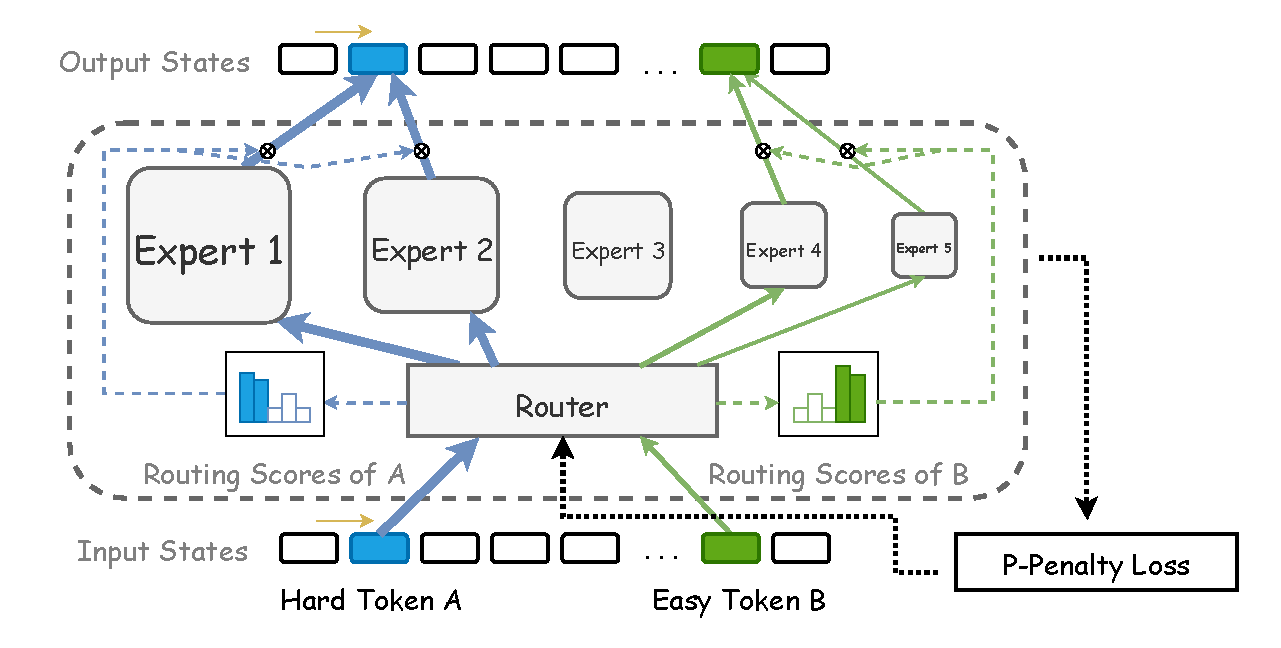
\includegraphics[width=0.9\linewidth]{figures/hmoe.pdf}
    \caption{HMoE模型为每个专家设置了不同的隐藏层维度\cite{Wang2024HMoEHM}。}
    \label{fig:hmoe}
\end{figure}

\paragraph{Grove MoE}
受到CPU计算架构中 big.LITTLE 设计的启发，Grove MoE\cite{Wu2025GroveMT}提出了一种新颖的专家组织方式（图\ref{fig:grovemoe}）。它将 $n$ 个基础专家分为 $g$ 个组，并为每个组分配一个共享的\textbf{伴随专家} (Adjugate Expert) $A_j$。当一个词元激活了某个组内的专家 $E_i$ 时，其最终输出由基础专家和其所在组的伴随专家的输出加权构成：
\begin{equation}
    \tilde{e}_i(x) = E_i(x) + \lambda A_j(x), \quad \text{其中 } E_i \in G_j
\end{equation}
这种设计的关键优势在于其动态计算分配机制。如果一个词元同时激活了同一组内的多个专家，那么共享的伴随专家 $A_j$ 的计算结果会被复用，只需计算一次。这种结构在不显著增加计算复杂度的前提下，高效地扩展了模型容量。此外，为了维持专家间的负载均衡，Grove MoE采用了\textbf{无辅助损失的负载均衡策略} (auxiliary-loss-free load balancing strategy)\cite{Wang2024AuxiliaryLossFreeLB,DeepSeekAI2024DeepSeekV3TR}。该方法不向总损失函数中添加负载均衡惩罚项，而是为每个专家的路由分数引入一个动态偏置项 (dynamic bias term)，通过直接更新该偏置项来最小化专家负载的不均衡，从而实现高效的训练。

\begin{figure}[h]
    \centering
    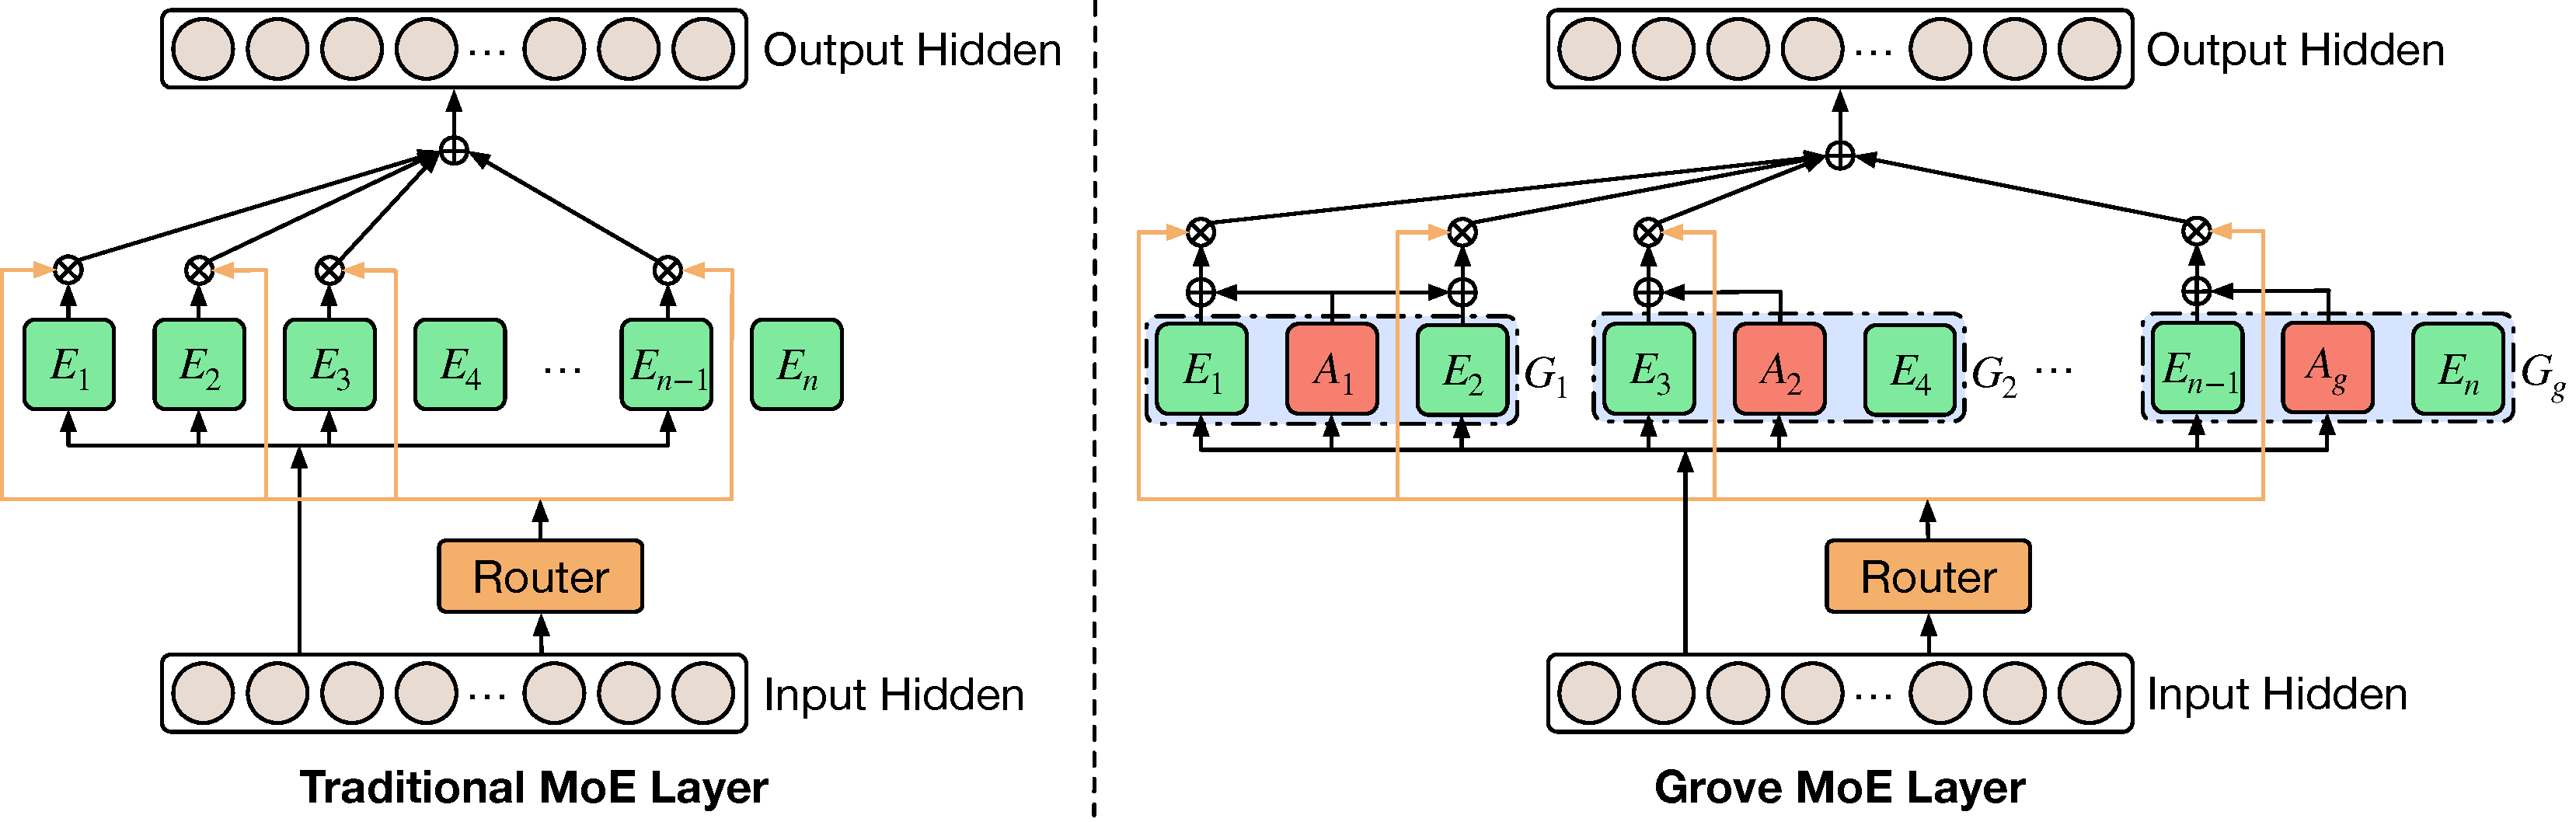
\includegraphics[width=1.0\linewidth]{figures/grovemoe.pdf}
    \caption{Grove MoE的架构\cite{Wu2025GroveMT}}
    \label{fig:grovemoe}
\end{figure}

% \section{专家网络的设计与约束}

% 这部分移到下面去，然后把帐结名字改成负混合专家模型的负载均衡

% aux loss那里提一下global aux loss的问题（引用deepseek v3, 还有阿里的那篇） 均衡性可以参考Aria里的图片，还有deepseek v3的

% 上面的部分补充图片

% \subsection{专家类型与同质性}
% 在当前主流的MoE模型中，如GShard\cite{·}、Switch Transformer\cite{Fedus2021}和Mixtral\cite{Jiang2023}，专家网络通常是\textbf{同质的}（Homogeneous）。这种设计的优势在于实现简单，易于利用专家并行（Expert Parallelism）进行分布式训练。模型的强大能力源于这些结构相同但参数独立的专家在海量数据上训练后，逐渐学习并形成了功能上的\textbf{专业化}（Specialization），这一点将在第五章详细讨论。

% \subsection{专家容量 (Expert Capacity)}
% 在硬件（如GPU/TPU）上高效地实现动态路由存在挑战，因为不同专家处理的词元数量在每个批次中是动态变化的，这会导致计算资源的闲置和同步开销。为了实现静态的计算图和高效的并行计算，GShard\cite{Lepikhin2020}引入了\textbf{专家容量}（Expert Capacity）这一关键的工程约束。专家容量定义了在单个前向传播批次中，每个专家能够处理的词元数量的上限。其计算方式通常为：
% \begin{equation}
%     \text{Capacity} = \left( \frac{\text{Tokens per batch}}{\text{num\_experts}} \right) \times \texttt{capacity\_factor}
% \end{equation}
% 其中，\texttt{capacity\_factor}是一个超参数（通常在1.25到2.0之间），用于为路由不均提供一定的缓冲空间。如果路由到一个专家的词元数量超过了其容量，那么多余的词元将被\textbf{丢弃}（Dropped）。这些被丢弃的词元不经过专家网络计算，其在MoE层的输出通过残差连接（Residual Connection）直接等于其输入。过高的词元丢弃率会损害模型性能，因此设计有效的负载均衡策略以最小化词元丢弃率，是MoE模型训练中的一个核心优化目标。

% \section{MoE模型的训练策略}

% \subsection{核心挑战：负载不均衡}
% 如前所述，MoE模型训练中最核心的挑战是\textbf{负载不均衡}（Load Imbalance）。在没有干预的情况下，Top-k路由器倾向于将大量词元发送给少数几个专家，形成一种“富者愈富”的马太效应。这种现象会导致训练效率低下、模型性能受损，以及大量专家参数得不到充分训练，造成模型容量的浪费。

% \subsection{经典的负载均衡策略：辅助损失函数}
% 为了缓解负载不均衡问题，Shazeer等人\cite{Shazeer2017}提出引入一个\textbf{辅助损失函数}（Auxiliary Loss Function），该方法被后续工作广泛采用。这个损失函数被加权后添加到模型的总损失中，专门用于惩罚不均衡的路由决策。对于一个包含 $T$ 个词元的批次，定义 $f_i$ 为路由到专家 $i$ 的词元比例，$\bar{P}_i$ 为专家 $i$ 从路由器获得的总门控权重之和。辅助损失 $L_{\text{aux}}$ 可以表示为：
% \begin{equation}
%     L_{\text{aux}} = \alpha \cdot \sum_{i=1}^{N} (f_i \cdot \bar{P}_i)
%     \label{eq:aux_loss}
% \end{equation}
% 这个损失函数通过最小化每个专家的词元分配比例和总路由权重的点积，来鼓励路由器将词元和路由权重都更均匀地分配给所有专家。超参数 $\alpha$ 控制了负载均衡与主任务损失（如交叉熵）之间的权衡。这一策略已被证明是训练稳定且高性能MoE模型的关键。

% \subsection{MoE的并行训练策略}
% 由于MoE模型巨大的参数量，其训练必须依赖高效的并行策略。除了标准的数据并行（Data Parallelism）外，GShard\cite{Lepikhin2020}开创性地提出了\textbf{专家并行}（Expert Parallelism）策略。在这种模式下，模型中的非MoE层参数（如自注意力模块）在所有计算设备上进行副本复制（类似数据并行），而 $N$ 个专家则被均匀地分配到不同的计算设备上。

% 在MoE层的前向和后向传播中，需要一次\texttt{All-to-All}的全局通信操作。具体来说，每个设备上的词元会根据本地路由器的决策，被发送到其目标专家所在的设备进行计算，计算完成后再通过一次\texttt{All-to-All}通信将结果传回原始设备。专家并行策略使得模型总参数量可以随着计算设备的增加而线性扩展，是成功训练万亿级别MoE模型的基石。
\section{混合专家模型的负载均衡}

混合专家模型通过引入稀疏激活的专家网络，极大地扩展了模型的参数容量，同时保持了计算量的相对恒定。然而，这种架构也带来了新的挑战，其中最核心的就是\textbf{负载均衡（Load Balancing）}问题。为了有效训练大规模混合专家模型，必须采用高效的并行策略和负载均衡机制。

\subsection{背景：专家并行与负载不均衡}
\label{sec:ep_and_lb}
由于混合专家模型巨大的参数量，单个计算设备（如 GPU/TPU）往往难以容纳，因此必须采用模型并行策略。其中，\textbf{专家并行（Expert Parallelism）}是专门为混合专家模型设计的核心并行方法\cite{Lepikhin2020GShardSG,Fedus2021SwitchTS}。

在专家并行策略中，模型的共享部分（如自注意力层）在所有设备上进行复制，而专家网络则被均匀地划分到不同的计算设备上。在训练的前向传播过程中，每个设备上的路由器会为本地的词元（token）批次做出路由决策。随后，通过一次高效的全局通信操作（通常是 All-to-All），需要由特定专家处理的词元被发送到持有该专家的相应设备上。计算完成后，再通过另一次 All-to-All 通信将结果发送回原始设备进行加权求和。

这种并行方式虽然极大地降低了单个设备的内存需求，但其效率高度依赖于路由器能够将词元均匀地分配给所有专家。如果路由决策出现倾斜，即大量词元被发送给少数几个“热门”专家，就会导致严重的\textbf{负载不均衡（Load Imbalance）}。这种不均衡会造成以下问题：
\begin{itemize}
    \item \textbf{计算资源浪费：} “热门”专家所在的设备将处理大量计算，而“冷门”专家所在的设备则处于空闲或等待状态，导致整体计算效率低下。
    \item \textbf{训练不足：} 大量专家参数得不到充分的训练，造成模型容量的浪费，最终损害模型性能。
    \item \textbf{通信瓶颈：} All-to-all 通信的开销与各设备间传输的数据量直接相关，不均衡的分配会加剧通信瓶颈。
\end{itemize}
因此，设计有效的负载均衡策略是成功训练高性能混合专家模型的关键。一个合理的衡量负载均衡程度的指标是\textbf{最大负载违规率（Maximal Violation, MaxVio）}\cite{Wang2024AuxiliaryLossFreeLB}，它用于量化专家负载的不均衡程度：
\begin{equation}
    \text{MaxVio} = \frac{\max_{i}(\text{Load}_i) - \overline{\text{Load}}}{\overline{\text{Load}}}
\end{equation}
其中，$\text{Load}_i$ 表示分配给第 $i$ 个专家的词元数量，$\overline{\text{Load}}$ 表示在完美均衡情况下的期望负载。MaxVio 值越小，表示负载越均衡。

\subsection{负载均衡的解决策略}
为了应对负载不均衡问题，学术界和工业界探索了多种策略，主要可以分为引入辅助损失函数、增加路由随机性和允许词元丢弃等。

\subsubsection{辅助负载均衡损失函数}
\label{sec:aux_loss}
最经典且广泛应用的策略是引入一个\textbf{辅助负载均衡损失函数（Auxiliary Load Balancing Loss）}\cite{Shazeer2017OutrageouslyLN,Lepikhin2020GShardSG}。这个损失函数被加权后添加到模型的总损失中，专门用于惩罚不均衡的路由决策。

Shazeer 等人\cite{Shazeer2017OutrageouslyLN} 在其开创性的工作中提出了一种形式，该损失函数鼓励所有专家获得同等的重要性。其核心思想是最小化专家重要性（importance，即批次内所有词元对该专家的门控值之和）分布的变异系数（coefficient of variation）：
\begin{equation}
    L_{\text{balance}} = w_{\text{balance}} \cdot \text{CV}(\textbf{Importance})^2
\end{equation}
其中 \textbf{Importance} 是一个向量，其第 $i$ 个元素是批次中所有词元路由到专家 $i$ 的门控值之和。

随后，在 GShard\cite{Lepikhin2020GShardSG} 和 Switch Transformer\cite{Fedus2021SwitchTS} 等工作中，一种更为常用的形式被提出并得到广泛应用。对于一个包含 $T$ 个词元的批次，该损失函数定义为所有专家 $i$ 的路由分配比例 $f_i$ 与总门控权重比例 $P_i$ 的点积之和：
\begin{equation}
    L_{\text{balance}} = \alpha \cdot N \sum_{i=1}^{N} (f_i \cdot P_i)
\end{equation}
其中，$N$ 是专家总数，$f_i$ 是路由到专家 $i$ 的词元数量占总词元数的比例，$P_i$ 是专家 $i$ 从路由器获得的总门控权重之和占批次总权重的比例。$\alpha$ 是一个超参数，用于控制负载均衡与主任务损失之间的权衡。这个损失函数通过最小化每个专家的词元分配比例和总路由权重的点积，来鼓励路由器将词元和路由权重都更均匀地分配给所有专家。这种方法已被证明是训练稳定且高性能的混合专家模型的关键。

\paragraph{设备级与通信级负载均衡损失}
在利用专家并行（Expert Parallelism）进行大规模分布式训练时，除了要考虑每个专家（Expert）的负载均衡，还需要考虑托管专家的计算设备（Device）的负载均衡，以避免部分设备计算过载而其他设备空闲。此外，设备间的通信开销也是一个关键瓶颈。为此，DeepSeek-V2 \cite{DBLP:journals/corr/abs-2405-04434} 等模型在经典负载均衡损失的基础上，引入了针对设备和通信的辅助损失函数。

\begin{itemize}
    \item \textbf{设备级负载均衡损失（Device-Level Balance Loss）}：该损失旨在确保每个设备处理的词元（Token）数量大致相等。假设有 $D$ 个设备，所有路由专家被划分到这 $D$ 个设备上。对于一个批次（Batch）的词元，设备 $d$ 的负载比例 $f_d$ 定义为路由到该设备上所有专家的词元数占总词元数的比例。类似地，设备 $d$ 的总门控权重比例 $P_d$ 是其上所有专家的门控权重之和占批次总权重之和的比例。设备级负载均衡损失可以定义为：
    \begin{equation}
        L_{\text{device}} = \alpha_{\text{device}} \cdot \sum_{d=1}^{D} (f_d \cdot P_d)
    \end{equation}
    其中 $\alpha_{\text{device}}$ 是一个超参数。这个损失函数鼓励模型将词元均匀地分配到所有设备上。

    \item \textbf{通信均衡损失（Communication Balance Loss）}：在分布式训练中，词元的表征（Representation）需要通过 All-to-All 通信操作发送到持有目标专家的设备上。如果某个设备需要接收大量来自其他设备的词元，就会成为通信瓶颈。通信均衡损失旨在均衡每个设备接收的词元数量。其形式与设备级负载均衡损失类似，但其优化的目标是每个设备\textbf{接收}的词元分布，从而保证设备间通信负载的均衡。
\end{itemize}

% 这里补一下v2的device aux loss

\subsubsection{随机路由}
为了从机制上促进负载均衡，研究者们也探索了在路由过程中引入随机性的方法。
\begin{itemize}
    \item \textbf{带噪声的 Top-k 路由：} Shazeer 等人\cite{Shazeer2017OutrageouslyLN} 提出，在计算出的路由 Logits送入 Top-k 选择逻辑之前，为其添加一个可学习的、与输入相关的噪声。
    \begin{equation}
        h_{\text{noisy}}(x)_i = (xW_g)_i + \text{StandardNormal}() \cdot \text{Softplus}((xW_{\text{noise}})_i)
    \end{equation}
    这种随机性可以打破路由决策的确定性，使得更多的专家有机会被激活。
    \item \textbf{随机丢弃专家：} 在 GShard\cite{Lepikhin2020GShardSG} 的 Top-2 路由中，引入了依照第二个专家的概率分数（即输出权重）随机丢弃该专家的策略。这种方法在一定程度上改善了负载均衡。
\end{itemize}
不过，由于随机路由可能给训练带来不稳定性，并增加推理部署时的不确定性，在当前的大语言模型中已较少被采用。

\subsubsection{专家容量与词元丢弃}
在硬件（如 GPU/TPU）上高效地实现动态路由存在挑战，因为不同专家处理的词元数量在每个批次中是动态变化的，这会导致计算资源的闲置和同步开销。为了实现静态的计算图和高效的并行计算，GShard\cite{Lepikhin2020GShardSG} 和 Switch Transformer\cite{Fedus2021SwitchTS} 引入了\textbf{专家容量（Expert Capacity）}这一关键的工程约束。

专家容量定义了在单个前向传播批次中，每个专家能够处理的词元数量的上限。其计算方式通常为：
\begin{equation}
    \text{Capacity} = \left( \frac{\text{Tokens per batch}}{\text{num\_experts}} \right) \times K \times \text{capacity\_factor}
\end{equation}
其中，$K$是每个词元路由到的专家数，capacity\_factor 是一个超参数（通常在 1.25 到 2.0 之间），用于为路由不均提供一定的缓冲空间。如果路由到一个专家的词元数量超过了其容量，那么多余的词元将被\textbf{丢弃（Dropped）}。这些被丢弃的词元不经过专家网络计算，其在混合专家模型层的输出通过残差连接（Residual Connection）直接等于其输入。过高的词元丢弃率会损害模型性能，因此设计有效的负载均衡策略以最小化词元丢弃率，是混合专家模型训练中的一个核心优化目标。

为了在硬件上高效地实现动态路由，除了设置专家容量和丢弃策略外，研究者们还设计了多种机制来管理路由过程。GShard \cite{Lepikhin2020GShardSG} 提出了一种\textbf{本地分组调度机制}。其核心思想是将一个训练批次中的所有词元均匀地划分为 $G$ 个组，每个专家的容量也被相应地分配到各个组中，每个组独立地限制专家容量。另一方面，在使用专家并行时，一个词元选择的多个专家可能分布在不同的计算设备上，这会产生 All-to-All 通信。当激活的专家数量较多时，通信开销会非常显著。为了直接从机制上限制通信开销，DeepSeek-V2 \cite{DBLP:journals/corr/abs-2405-04434} 提出了\textbf{设备受限路由（Device-Limited Routing）}策略。该策略为每个词元的路由增加了一个约束：其选择的目标专家必须位于不超过 $M$ 个设备上（$M$ 是一个较小的常数，例如3）。具体的路由过程分为两步：首先，对于一个词元，模型会计算其与所有专家的亲和度分数，并找出得分最高的专家所在的 $M$ 个设备；然后，模型仅在这 $M$ 个设备上的专家中执行 Top-k 选择。这种方法直接限制了每个词元需要通信的目标设备数量，从而有效控制了通信带宽，降低了训练延迟。